\chapter{Measurement of Neutral Current Quasielastic
Interactions with Super-Kamiokande Gadolinium Upgrade}
\label{chp:ncqegd}

This chapter is dedicated to the main analysis of this thesis, the motivation for which is to constrain the SRN background by looking at the atmospheric neutral current quasi-elastic (NCQE) interactions of atmospheric neutrinos which form a significant background for this SRN search, as the prompt and delayed signal of the NCQE interaction mimics that of the SRN. Previously the NCQE neutron tag has searched for the 2.2 MeV photon from neutron capture on hydrogen. With the recent addition of 0.026\% gadolinium sulphate octahydrate to Super-Kamiokande, this allows for improved neutron detection due to the higher energy gamma cascade signal of neutron capture on gadolinium of 8 MeV. At energies close to the atmospheric peak, the NCQE interaction cross sections can be evaluated using T2K beam neutrinos. This analysis will present the status of the improved neutron tag from SK-Gd, its impact on the measurement of NCQE in T2K and the improvements to the SRN background measurement.

There are many stages to this analysis, which are shown in Figure \ref{fig:analysis_flowchart}, where the ``neutron tagging'' stage occurs via two methods. Previous NCQE neutron-tagging analyses used a method for neutron tagging which will be referred to as ``legacy NTag code'', but in 2020 the Super-K collaboration decided to proceed to use a new, more compact and streamlined version of the neutron tagging code, which combines most of these stages into one piece of software. This will be referred to As``current NTag code'', and this is shown in Figure \ref{fig:analysis_flowchart} as well. The red arrows in Figure \ref{fig:analysis_flowchart} show the steps in the analysis prcoedure using the legacy NTag code which have been assimilated into the new NTag code.

\begin{figure}
    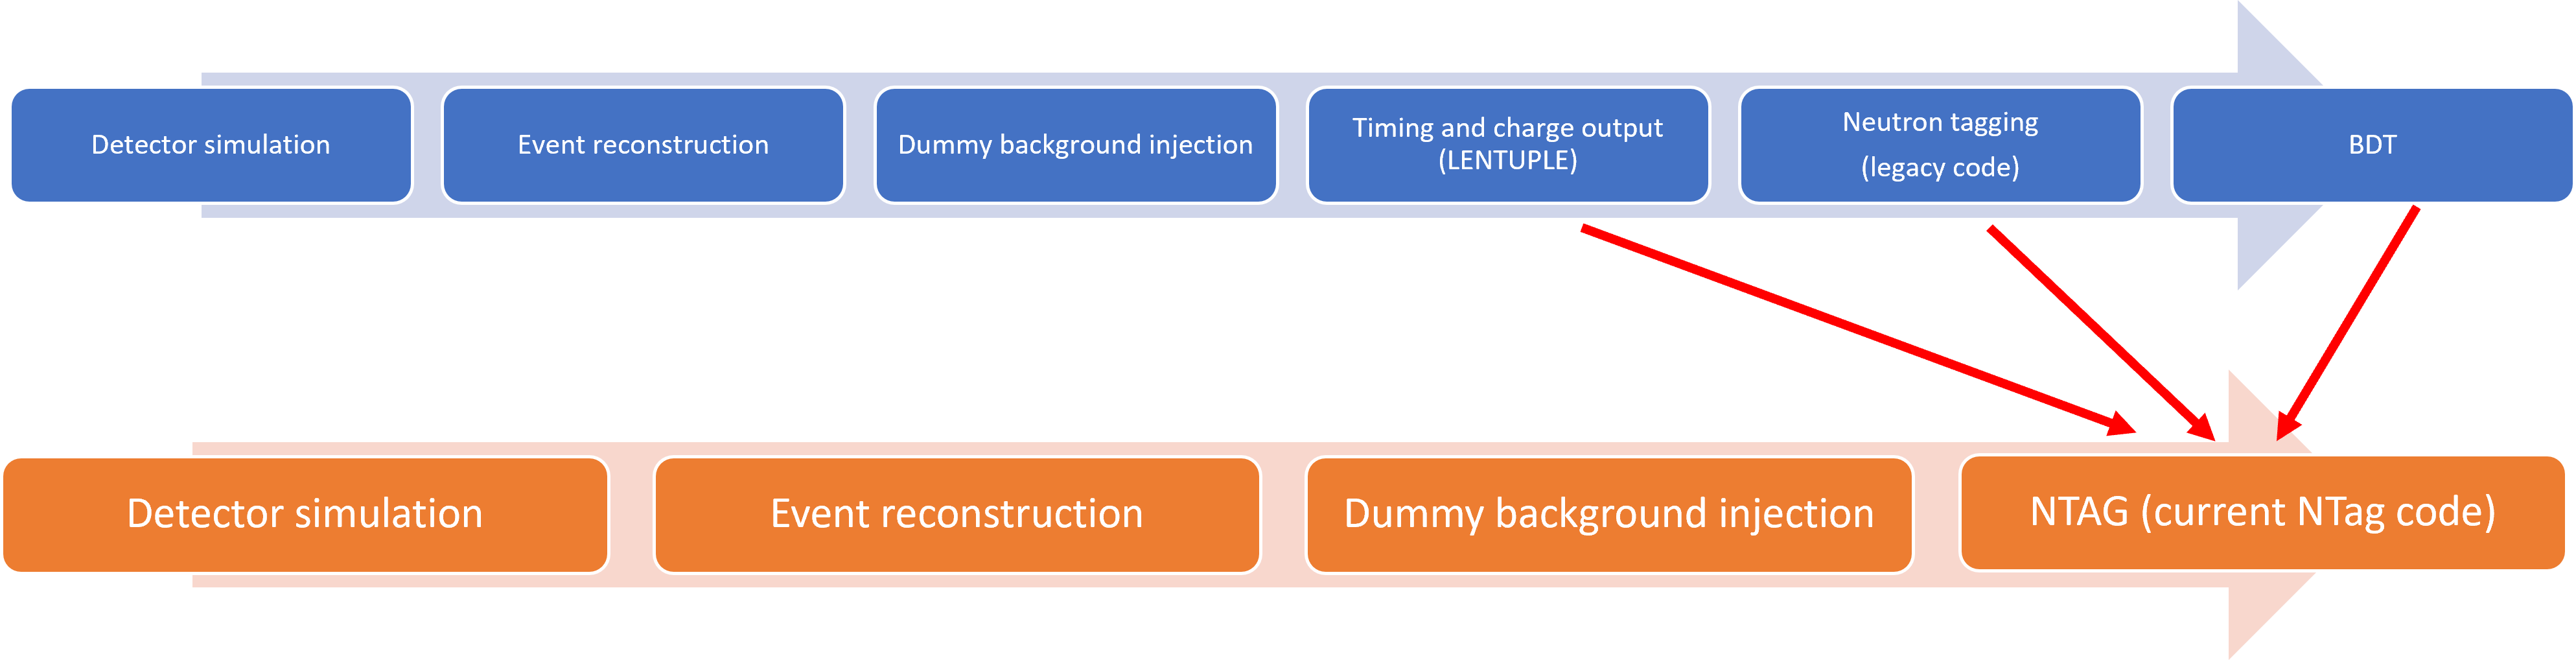
\includegraphics[width=\textwidth]{Figures/analysis_flowchart.png}
    \caption{Flowchart showing the stages in this analysis for both the analysis which used the legacy Ntag code (blue) and the current NTag code (orange).}
\label{fig:analysis_flowchart}
\end{figure}

The main differences between the legacy and new NTag code lie in the neutron tagging algorithm stage, especially regarding variables used to classify the tagged neutron candidates which will be discussed in further detail later on. A large part of this analysis was to ensure that the legacy and new NTag code produced the same information regarding the prompt event and also for the Monte Carlo truth information regarding the neutrons. 



\section{Event Simulation}

This chapter discusses details about the event simulation, specifically the software used and the way neutrino interactions are simulated in order to produce Monte Carlo. Table \ref{table:software} summarises all the software used in this analysis. 


\begin{table}
$$
\begin{array}{ll}
\hline \text { Name } & \text { Version } \\
\hline \text { Flux } & 13 \text { a tuning v4.0 } \\
\text { NEUT } & 5.3 .3 \\
\text { SKDETSIM-SKGd } & \text { ANNRI-Gd model } \\
\text { Geant } & 4.10.05.p01 \\
\text { T2KReWeight } & \text { v1r23 } \\
\text { GENIE } & \text { R2-12-10 } \\
\hline
\end{array}
$$
\caption{Software versions used in analysis}
\label{table:software}
\end{table}

\subsection{Neutrino flux}

The neutrino beam flux used in this analysis is 13a tuning v4.0, taken from the NA61/SHINE fixed target experiment at CERN \cite{vladisavljevic_constraining_2018}.  The NA61/SHINE experiment provides hadron production measurements for T2K and other long baseline experiments, and measures the yield of charged hadrons from a proton beam fired at a thin graphite target (2 cm long) and a T2K replica graphite target (90 cm long). From this experimental data, Monte Carlo simulations of the neutrino flux are predicted. The oscillation effect on the neutrino flux needs to be considered after choosing which flux to use, and although the neutrino-oxygen NCQE cross section does not depend on flavour (and therefore neutrino oscillation affects would have no impact on a fully pure NCQE sample) there is a small amount of charged current events which seep into the NCQE sample, and oscillation weights need to be applied to the charged current events in the sample. Monte Carlo reweighting takes care of this issue by assuming that they are all muon neutrino or muon anti-neutrino events, due to the fact that the number of electron neutrino events in FHC mode would be negligible.

\subsection{Primary interaction}

The interaction between the incoming neutrino event and an Oxygen nucleus, and it's consequent de-excitation is modelled by NEUT, which produces a vector of primary particles. Because these are primary particles, they do not take into consideration all the particles produced from the detector response, i.e. the secondary particles produced from the interactions within the medium of the detector, in our case, water doped with gadolinium sulphate octahydrate. The way NEUT treats the interaction between a nucleus and a neutrino for the case of a neutrino interaction with a $16_{O}$ isotope is shown in Equation \ref{eq:neutrinonuc}. 

\begin{equation}
    \sigma\left(\nu^{16} \mathrm{O}\right)=\sum_{i=1}^{8} \sigma_{\mathrm{p}}\left(p_{i}^{(\mathrm{p})}\right)+\sum_{j=1}^{8} \sigma_{\mathrm{n}}\left(p_{j}^{(\mathrm{n})}\right)+\sigma(2 p 2 h)    
\label{eq:neutrinonuc}    
\end{equation}

Here $\sigma_{p}$ and $\sigma_{n}$ are the neutrino-proton cross section and the neutrino-neutron cross section respectively, and these cross-sections are dependent on the momenta of the protons and neutrons in the model, and therefore on the choice on nuclear model. The Benhar Spectral Function (SF) is used by NEUT as the nuclear model for NCQE interactions, and for CCQE interactions the Smith-Moniz relativistic Fermi Gas (RFG) model is used \cite{benhar_electron-_2005}, with 2p2h interactions included for these interactions. 

\begin{figure}
    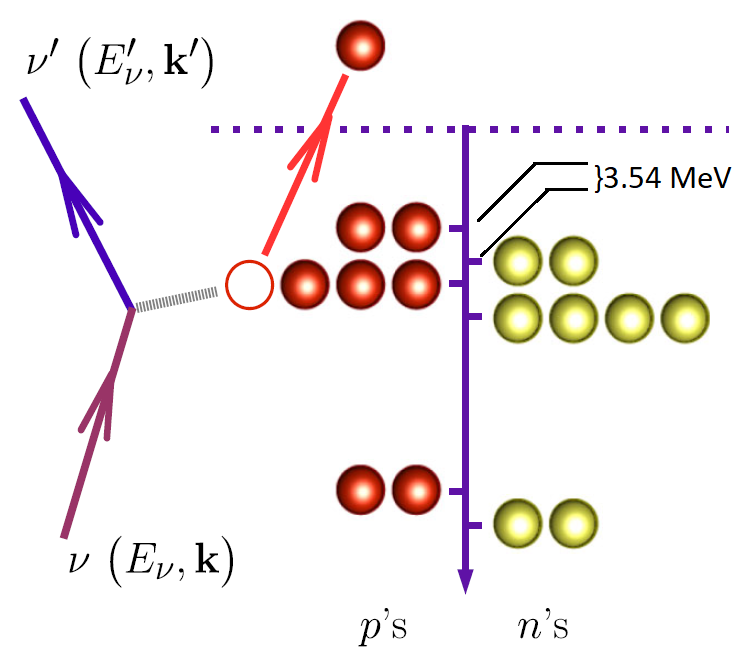
\includegraphics[width=\textwidth]{Figures/ncqebenharspectral.png}
    \caption{Representation of NC neutrino scattering off $16_{O}$ with protons on the left hand side and neutrons on the right arranged according to the shell model. }
\label{fig:ncqebenharspectral}
\end{figure}

The lowest rung of nucleons in Figure \ref{fig:ncqebenharspectral} is the $s_{1/2}$, with $p_{3/2}$ above this level and $p_{1/2}$ above that. The protons in these rungs have removal energies of 12.1 MeV, 18.4 MeV and 42 MeV respectively, and due to neutron levels being more tightly bound, these have an extra removal of 3.24 MeV compared to their proton counterparts. The shell model is imperfect due to how it allocates the probablity of $16_{O}$ transitioning to the possible nucleon states. In the shell model, probabilities are allocated by counting the number of nucleons in each energy level and assigning probailities according to how many there are. In Figure \ref{fig:ncqebenharspectral} it can be seen that the $p_{3/2}$ state has double the number of nucleons compared to the $s_{1/2}$ model and therefore double the probability of transition is assigned for the $p_{3/2}$ state, and the probability of transitioning to any other state is assigned to be 0, because in the shell model they don't even exist. The Benhar Spectral Function model however is complex and is tuned using electron-nucleus scattering data. The model used in this analysis is a modified version of the Benhar Spectral Function model, where the case of other transition states is dealt with by merging the "others'' state into the $s_{1/2}$ state. Table \ref{table:transitionprob} gives the probabilities of transition to different states for different models. 

\begin{table}
$$
\begin{array}{ccccc}
\hline & \left(\mathrm{s}_{1 / 2}\right)^{-1} & \left(\mathrm{p}_{3 / 2}\right)^{-1} & \left(\mathrm{p}_{1 / 2}\right)^{-1} & \text { others } \\
\hline \text { Shell model } & 0.25 & 0.5 & 0.25 & 0 \\
\text { Spectral Function } & 0.1055 & 0.3515 & 0.158 & 0.385 \\
\text { This analysis } & 0.4905 & 0.3515 & 0.158 & 0 \\
\hline
\end{array}
$$
\caption{Transition probabilities for different models and states}
\label{table:transitionprob}
\end{table}

\subsection{Detector response and interactions in the detector medium}

Prior analyses to this used SKDETSIM (Super-Kamiokande Detector Simulator) to simulate the trajectories of particles through the water in Super-Kamiokande and output detector response MC. This analysis uses SKDETSIM-SKGd to propogate the particles, due to the requirement of needing gadolinium sulphate present in the simulation. The particular isotopes of gadolinium used in the simulation are $155_{Gd}$ and $157_{Gd}$ due to their excellent thermal neutron capture cross sections. Table \ref{table:gdtable} shows the relative abundance of various gadolinium isotopes inside natural gadolinium and their associated thermal neutron capture cross sections.

\begin{table}
$$
\begin{array}{rcc}
\hline \text { Isotope } & \text { Abundance }[\%] & \text { Cross-section[b] } \\
\hline{ }^{152} \mathrm{Gd} & 0.200 & 735 \\
{ }^{154} \mathrm{Gd} & 2.18 & 85 \\
{ }^{155} \mathbf{Gd} & \mathbf{1 4 . 8 0} & \mathbf{6 0 9 0 0} \\
{ }^{156} \mathrm{Gd} & 20.47 & 1.8 \\
{ }^{157} \mathbf{Gd} \mathbf{d} & \mathbf{1 5 . 6 5} & \mathbf{2 5 4 0 0 0} \\
{ }^{158} \mathrm{Gd} & 24.84 & 2.2 \\
{ }^{160} \mathrm{Gd} & 21.86 & 1.4 \\
\hline
\end{array}
$$
\caption{Abundance and thermal neutron capture cross section of various isotopes of Gadolinium}
\label{table:gdtable}
\end{table}

As can be seen in Table \ref{table:gdtable}, not only are ${ }^{155} \mathrm{Gd}$ and ${ }^{157} \mathrm{Gd}$ the most abundant isotopes, they also have extremely high neutron capture cross sections compared to the other isotopes. Equation \ref{eq:gdisotopecaptureeq} shows the neutron capture on both of these isotopes, and the energy of the subsequent gamma rays.

\begin{equation}
\begin{split}
 {n}+{ }^{155} \mathrm{Gd} \rightarrow{ }^{156} \mathrm{Gd}^{*} \rightarrow{ }^{156} \mathrm{Gd}+\gamma  (8.536 MeV)\\
 {n}+{ }^{157} \mathrm{Gd} \rightarrow{ }^{158} \mathrm{Gd}^{*} \rightarrow{ }^{158} \mathrm{Gd}+\gamma  (7.937 MeV)
\end{split}
\label{eq:gdisotopecaptureeq}    
\end{equation}




It is important to therefore model the gamma ray emission spectra from both of these isotopes. The model used by SKDETSIM-SKGd is the ANNRI-Gd model. This uses gamma energy spectrum data from the germanium spectrometer at the ANNRI (Accurate Neutron Nucleus Reaction Measurement Instrument) experiment. This experiment uses the incoming pulsed neutron beam from the Japan Spallation Neutron Source (JSNS) at the Material and Life Science Experimental Facility (MLF) of J-PARC. After a 300 kW beam of protons from the JSNS facility hits a target of mercury and produces neutrons, this neutron beam hits an enriched ${ }^{155} \mathrm{Gd}$ target or a ${ }^{nat} \mathrm{Gd}$ film. The ANNRI spectrometer is placed 21.5 m away from the neutron beam source, with two cluster detectors on either side of the neutron capture target material, which is 13.4 cm away from each cluster detector. Surrounding the target, there are also 8 co-axial germanium detectors. The schematic for the ANNRI-Gd experiment is shown in Figure \ref{fig:annrigd}.

\begin{figure}

        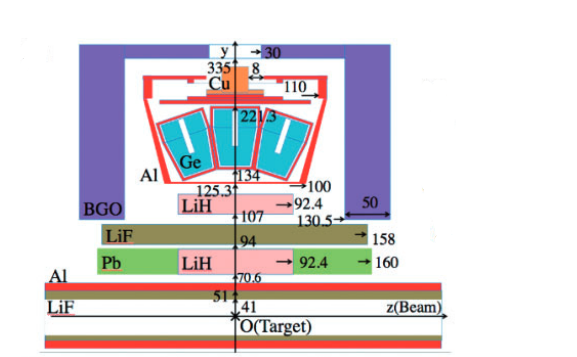
\includegraphics[width=\textwidth]{Figures/annrigd.png}
        \caption{Schematic of the ANNRI Ge spectrometer (dimensions in mm). The beam pipe along with one of the Ge cluster detectors (light blue) is shown. The shaded purple area are the anti-coincidence shields made of bismuth-germanium-oxide (BGO) crystals.}
        \label{fig:annrigd}
    
\end{figure}

By defining how many Germanium crystals were hit and how many neighbouring crystal recieved gamma ray hits, values of H (hit number) and M (multiplicity) can be assigned in order to classify the events. After selecting for neutron energy and subtracting the background, the events remaining were seperated into samples based on their H and M vales. Figure \ref{fig:annrigdenergyspectra} shows the energy spectra for different multiplicity values (left) and hit values (right) from one of the germanium crystals in the ANNRI spectrometer. 

\begin{figure}
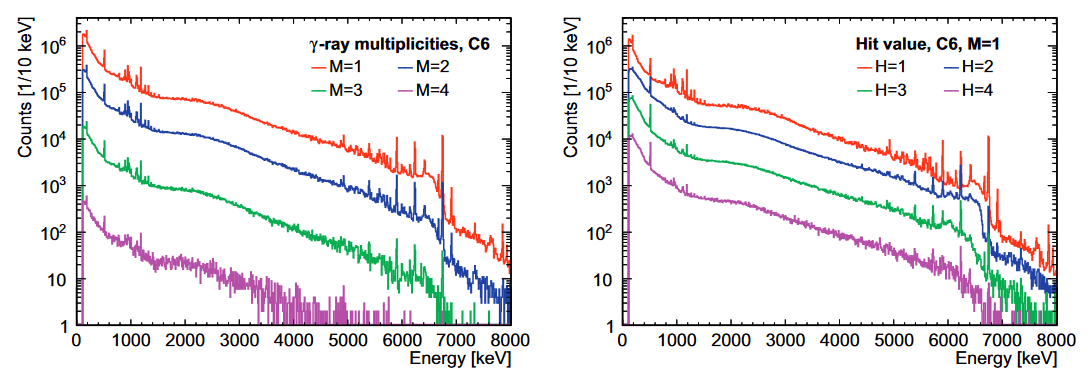
\includegraphics[width=\textwidth]{Figures/annrigdenergyspectra.png}
\caption{Energy spectra for thermal neutron capture on ${ }^{157} \mathrm{Gd}$ energy spectra for different multiplicity values (left) and hit values (right) from one of the germanium crystals in the ANNRI spectrometer.}
\label{fig:annrigdenergyspectra}
\end{figure}

One of the key differences between the default Geant4 model for thermal neutron capture on Gadolinium and the ANNRI-Gd model is how it conserves energy: the photon evaporation model conserves only the final sum of energy for the captured event, but performs poorly when modelling the gamma-ray energy on an individual event by event basis. One way the ANNRI-Gd model combats this is by seperately describing the continuous and discrete peaks in Figure \ref{fig:annrigdenergyspectra}, where the discrete peaks are shown as spikes below 1500 keV and above 4500 keV. These come from the different ways in which gadolinium de-excites after thermal neutron capture. The continuous spectrum in the plots in Figure \ref{fig:annrigdenergyspectra} show the de-excitation of ${ }^{158} \mathrm{Gd}^{*}$ in multiple steps, producing multiple low energy gamma rays, which accounts for about 93\% of the spectrum. The discrete spikes in the spectra come from a two-step cascade, which produces a high energy gamma ray instead, accounting for the remaining 7\% of the spectrum.
Figure \ref{fig:continousdiscrete} shows the continuous and discrete components of the ANNRI-Gd MC, along with data from the experiment. Figure \ref{fig:annrigdmodelcompare} shows ratio plot of data and MC for the GLG4sim model, the default Geant4 photon evaporation model and the ANNRI-Gd model: here it is clear the ANNRI-Gd model fits the data better than the other two models, especially at energies above 3500 keV. 

\begin{figure}
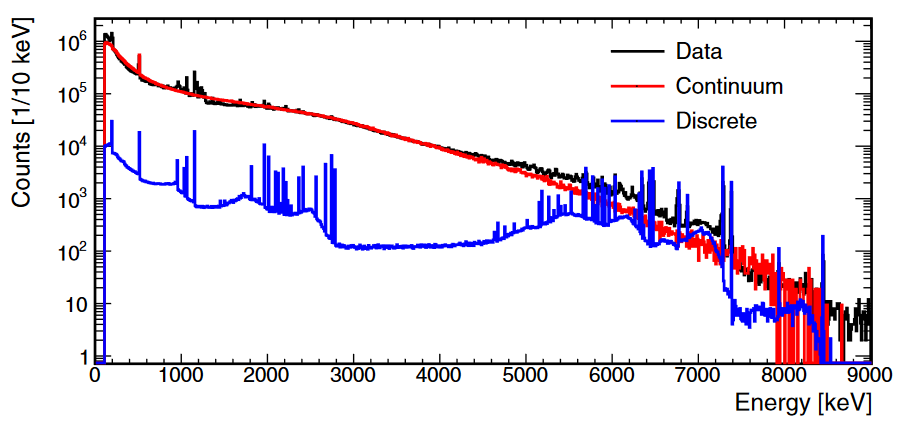
\includegraphics[width=\textwidth]{Figures/continousdiscrete.png}
\caption{Energy spectra for the ANNRI-Gd model broken down into its continous and discrete components along with data from the ANNRI-Gd experiment.}
\label{fig:continousdiscrete}
\end{figure}

\begin{figure}
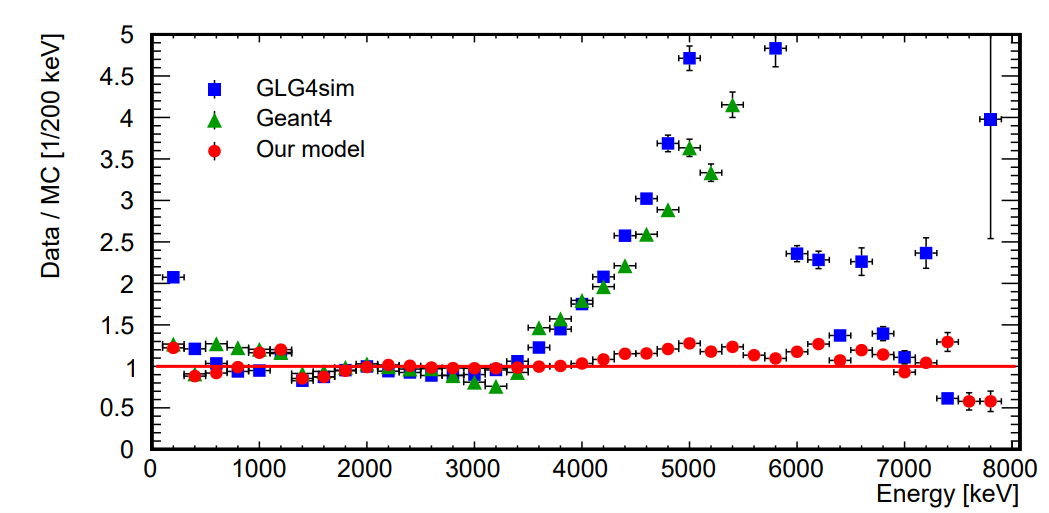
\includegraphics[width=\textwidth]{Figures/annrigdmodelcompare.png}
\caption{Comparison between neutron capture MC models and data.}
\label{fig:annrigdmodelcompare}
\end{figure}


\section{Event Reconstruction}
\subsection{Bonsai output reconstruction quantities}

Due to this analysis looking specifically at the low energy region, a fitter specific to low energies (called LOWFIT) is used to reconstruct events. Both MC and data neutrino events undergo a reconstruction phase, where the low-energy fitter BONSAI is applied to the event, which is discussed in Chapter 2. This reconstruction is carried out using timing and cable information, however charge information is omitted. The ouput of BONSAI gives information which will be used in the reduction phase of the data and allow for the selection of the NCQE sample. The following quantities comprise the BONSAI output, the first two being helpful spectator variables and the latter five constituting parameters which are used in the reduction phase of the analysis, from which the neutrino NCQE sample is determined.\\

\noindent
\underline{1. Neutrino vertex direction}\\
\noindent
This vector points towards the direction which is an average over all the Cherenkov cone axes which are produced, due to there being multiple leptons induced in the interaction.

\noindent
\underline{2. Neutrino vertex position}\\
\noindent 
The reconstructed location of the neutrino interaction event.

\noindent
\underline{3. Reconstructed energy}\\
\noindent 
In line with the standard SK low energy analysis definition, this energy is simply the reconstructed energy with the 0.511 MeV electron mass omitted. The range for Erec in this variable is 3.49 MeV to 29.49 MeV - the estimated kinetic energy under the hypothesis that the event is a singular electron.

\noindent
\underline{4. Dwall}\\
\noindent 
This variable gives the minimum distance of the neutrino vertex position from the closest wall of the Super-Kamiokande detector.

\noindent
\underline{5. Effwall}\\
\noindent 
Thus variable gives the distance between the neutrino vertex position and the closest wall, but moving back from the vertex position along the neutrino vertex direction vector.

\noindent
\underline{6. Vertex direction and goodness coefficient}\\
\noindent 
The coefficient $ovaQ$ (defined in Equation \ref{eq:ovaq}) describes the quality of the vertex reconstruction. It consists of two parameters $g^2_{vtx}$ and $g^2_{dir}$ where the former describes the goodness of the vertex which is based on PMT hit timings, and increases the sharper an event is in time. The latter is the directional goodness and measures the azimuthal uniformity in the ring pattern produced by the Cherenkov cone, which decreases the more uniform an event is in space. As a result of this, $ovaQ$ increases the more uniform and sharp in time an event is.

\begin{equation}
    \text { ova } Q=g_{\text {vtx }}^{2}-g_{\text {dir }}^{2}
    \label{eq:ovaq}
\end{equation}

$g_{vtx}$ is calculated using a fit of the PMT timing distribution and using the hit times of the PMT it is defined as in Equation\ref{eq:vertex_goodness}.

\begin{equation}
g_{\mathrm{vtx}}=\frac{\sum_{i} w_{i} \mathrm{e}^{-\frac{1}{2}(\frac{\Delta t_{i}}{\sigma})^{2}}}{\sum_{i} w_{i}} \text { with } w_{i}=-\frac{1}{2}(\frac{\Delta t_{i}}{\omega})^{2}
\label{eq:vertex_goodness}
\end{equation}

Here $\sum_{i} w_{i}$ is the weight given to the i-th hit PMT for the reduction of dark noise, where $\omega$ has a value of 60ns. $\sigma$ has a value of 5ns which is used to test the goodness, and as a result, a sharp timing distribution produces a large vertex goodness. $g_{dir}$ is calculated by looking at how spatially uniform the hit PMTs are around the reconstructed neutrino vertex direction. In order to quantify this uniformity, the Kolmogorov-Smirnov (KS) test is used as in Equation \ref{direction_goodness}.

\begin{equation}
    \mathrm{g}_{\mathrm{dir}}=\frac{\max _{i}\{\angle_{\mathrm{uni}}(i)-\angle_{\mathrm{data}}(i)\}-\min _{i}\{\angle_{\mathrm{uni}}(i)-\angle_{\mathrm{data}}(i)\}}{2 \pi}
\label{direction_goodness}
\end{equation}

where $\angle_{\mathrm{data}}(i)$ is the azimuthal angle of i-th hit real PMT included in the number of hits in 50ns. $\angle_{\mathrm{uni}}(i)=2 \pi i / N_{50}$ is the azimuthal angle of the i-th virtual PMT hit, but only when uniform distribution of the hits is assumed. As the uniformity of the hit pattern increases, the goodness decreases. 
 


\noindent
\underline{7. Cherenkov angle $\theta_{C}$}\\
\noindent
 For relativistic electrons in water, the value of the Cherenkov opening angle is $\approx 41\degree$, due to the relation: 

 \begin{equation}
\cos \theta_{\mathrm{Cherenkov}}=\frac{1}{n\beta}
\label{cherenkov_angle}
\end{equation}
 
where $\beta = v/c \approx 1$ and $n$ is the refractive index of water, 1.33. However due to other particles in the simulation, such as protons or muons, the Cherenkov cone is expected to be narrower, or if multiple leptons are present, the Cherenkov cones will be less distinct and more spread out, leading to deviations from the 41\degree value. 

\subsection{Comparison of BONSAI reconstruction output variables between SKDETSIM versions}

The BONSAI reconstruction output variables were compared between three versions of SKDETSIM, the version used in the previous NCQE neutron capture on hydrogen only analysis, with no neutron capture on Gd implemented (black), the SKDETSIM-SKGd photon-evaporation model mentioned in the previous section (red), and the SKDETSIM SK-Gd ANNRI-Gd model (green). Figure \ref{fig:bonsai_reconstruction_compare} shows the comparison of these models for the output BONSAI variables Erec, dwall, effwall, ovaQ, and $\theta_C$, where the y-axis shows the number of events.

\begin{figure}[!htbp]
    \centering
    
    \caption{Comparisons of BONSAI output variables bewteen SKDETSIM versions} \label{fig:bonsai_reconstruction_compare} 
    
    \subfloat[]{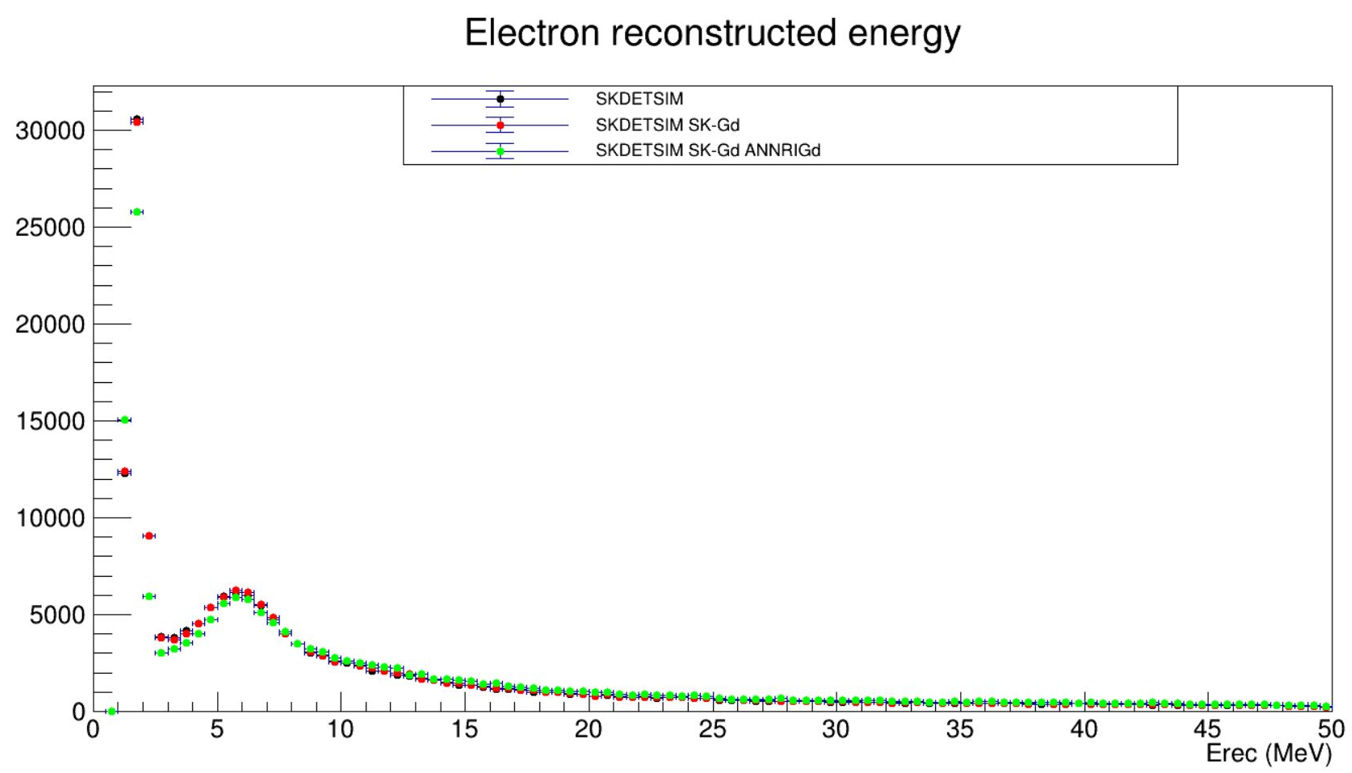
\includegraphics[width=0.49\textwidth]{Figures/erec_compare.PNG}} \hfill
    \subfloat[]{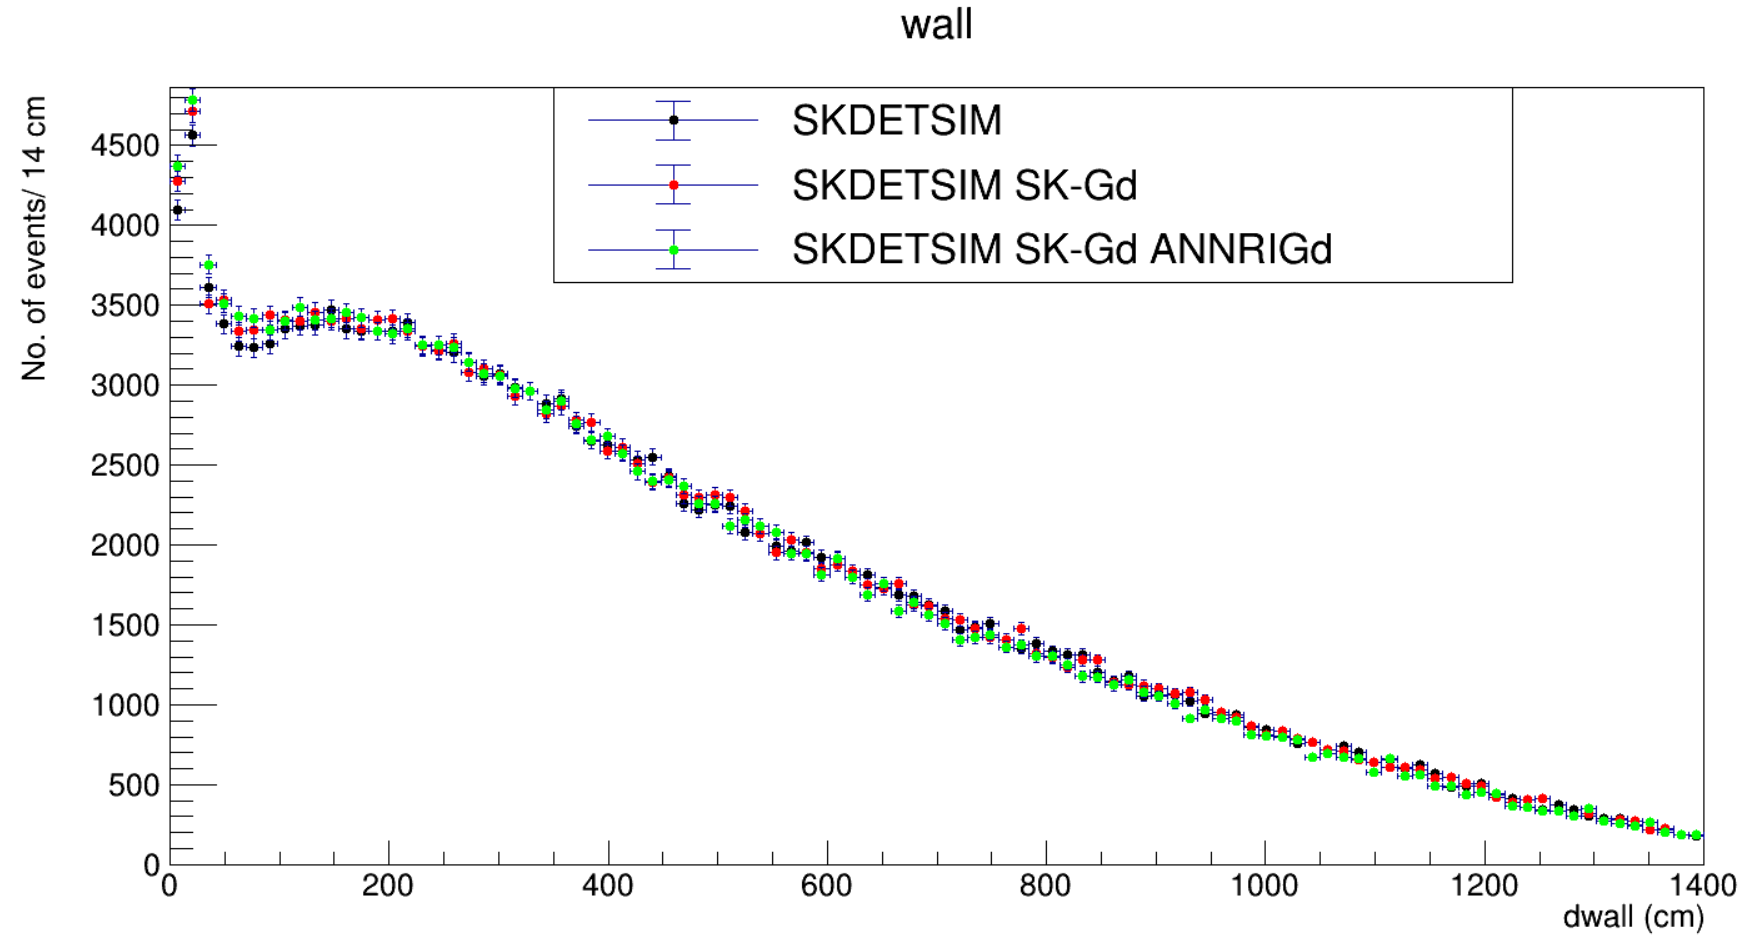
\includegraphics[width=0.49\textwidth]{Figures/dwall_compare.PNG}} \par
    \subfloat[]{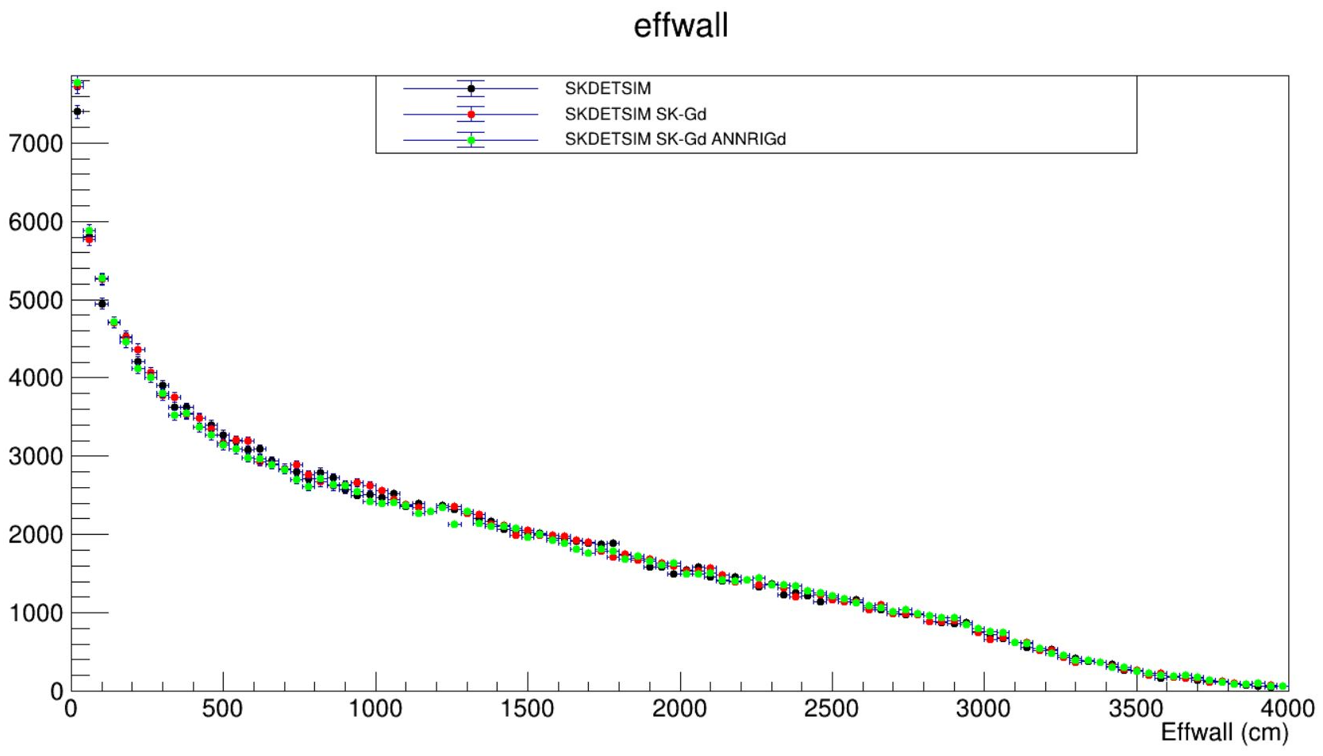
\includegraphics[width=0.49\textwidth]{Figures/effwall_compare.PNG}} \hfill
    \subfloat[]{\includegraphics[width=0.49\textwidth]{Figures/ovaQ_compare.PNG}} \par
    \subfloat[]{\includegraphics[width=0.49\textwidth]{Figures/thetaC_compare.PNG}} \hfill    
\end{figure}

To ensure correct implementation of the ANNRI-Gd model, ensuring the BONSAI output variables were similar between these SKDETSIM versions was important as the Gadolinium model should only effect the neutron capture in the simulation, not the output from event reconstruction of the neutrino interaction vertex. As can be seen in Figure \ref{fig:bonsai_reconstruction_compare}, this holds true for Erec, dwall, effwall and $\theta_C$, but not for the vertex and goodness coefficient ovaQ, where the ANNRI-Gd model differs for ovaQ between -0.05 and 0.15 compared to the SKDETSIM and SKDETSIM photon-evaporation model. To investigate this difference further, distributions of the vertex goodness and the directional goodness which make up ovaQ (according to Equation \ref{eq:ovaq}) were also checked, shown in Figure \ref{fig:ovaq_compare}.

\begin{figure}[!htbp]
    \centering
    
    \caption{Comparisons of vertex goodness and directional goodness between SKDETSIM versions} \label{fig:ovaq_compare} 
    
    \subfloat[]{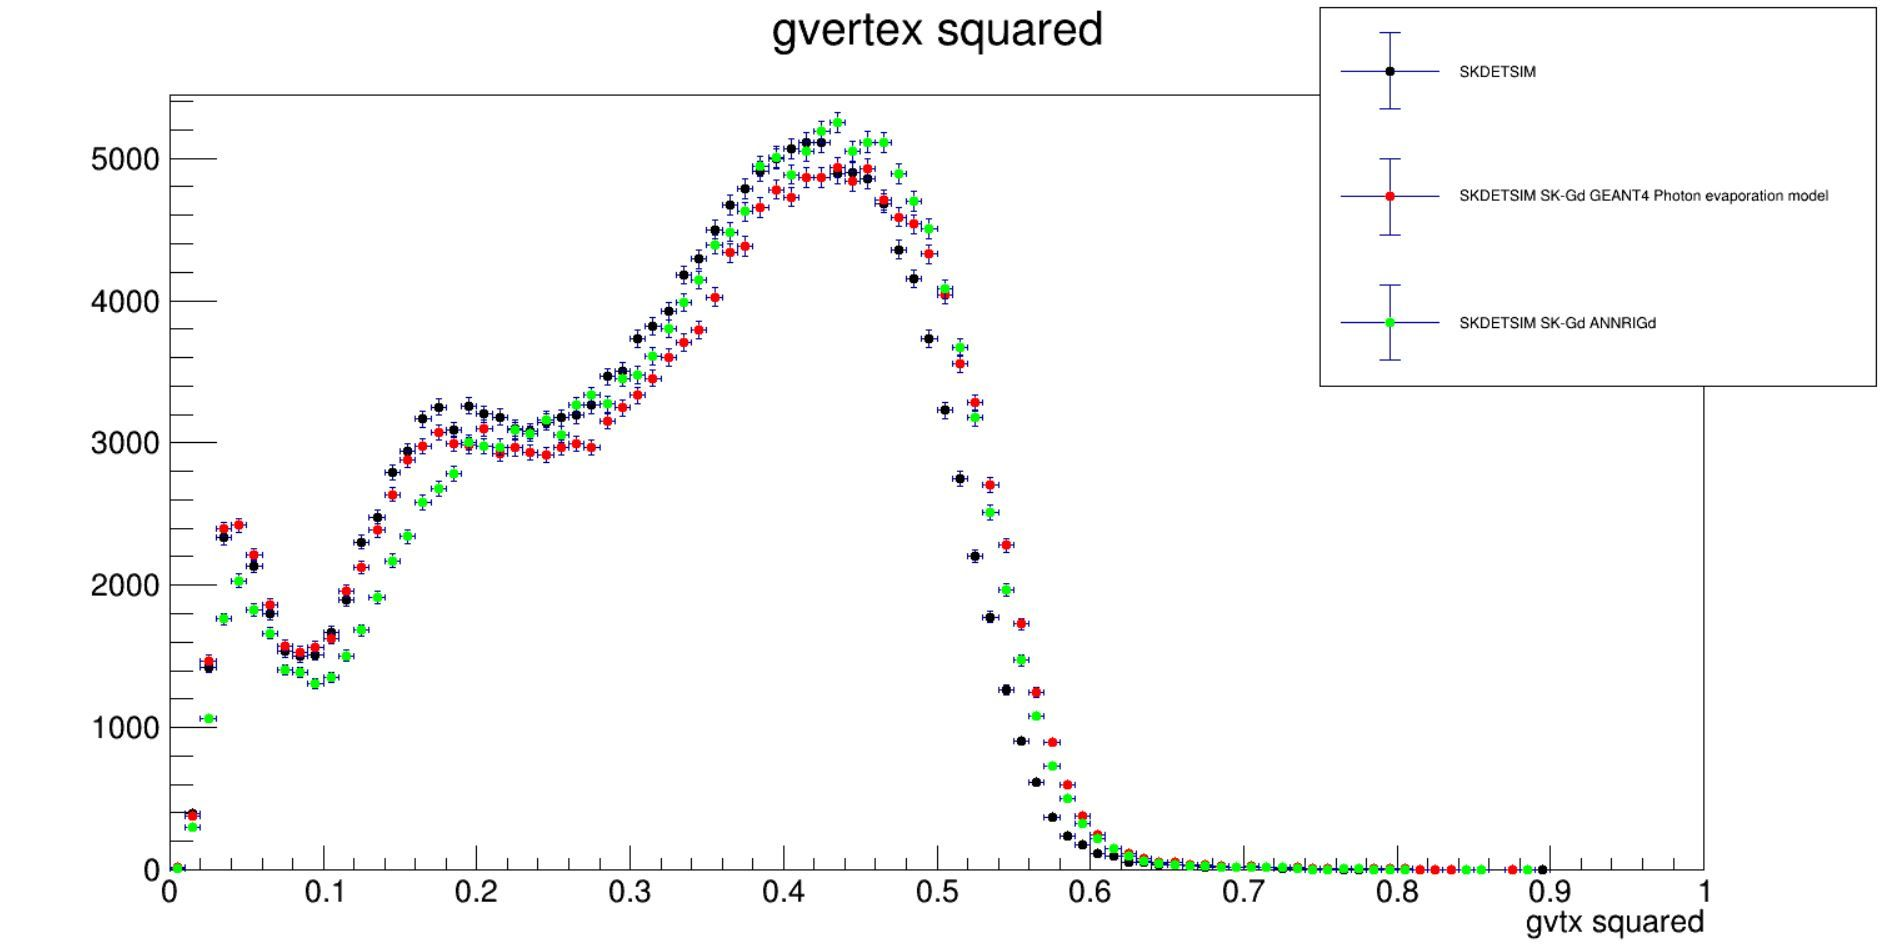
\includegraphics[width=0.49\textwidth]{Figures/gvtx_squared.JPEG}} \label{fig:gvtx_squared} \hfill 
    \subfloat[]{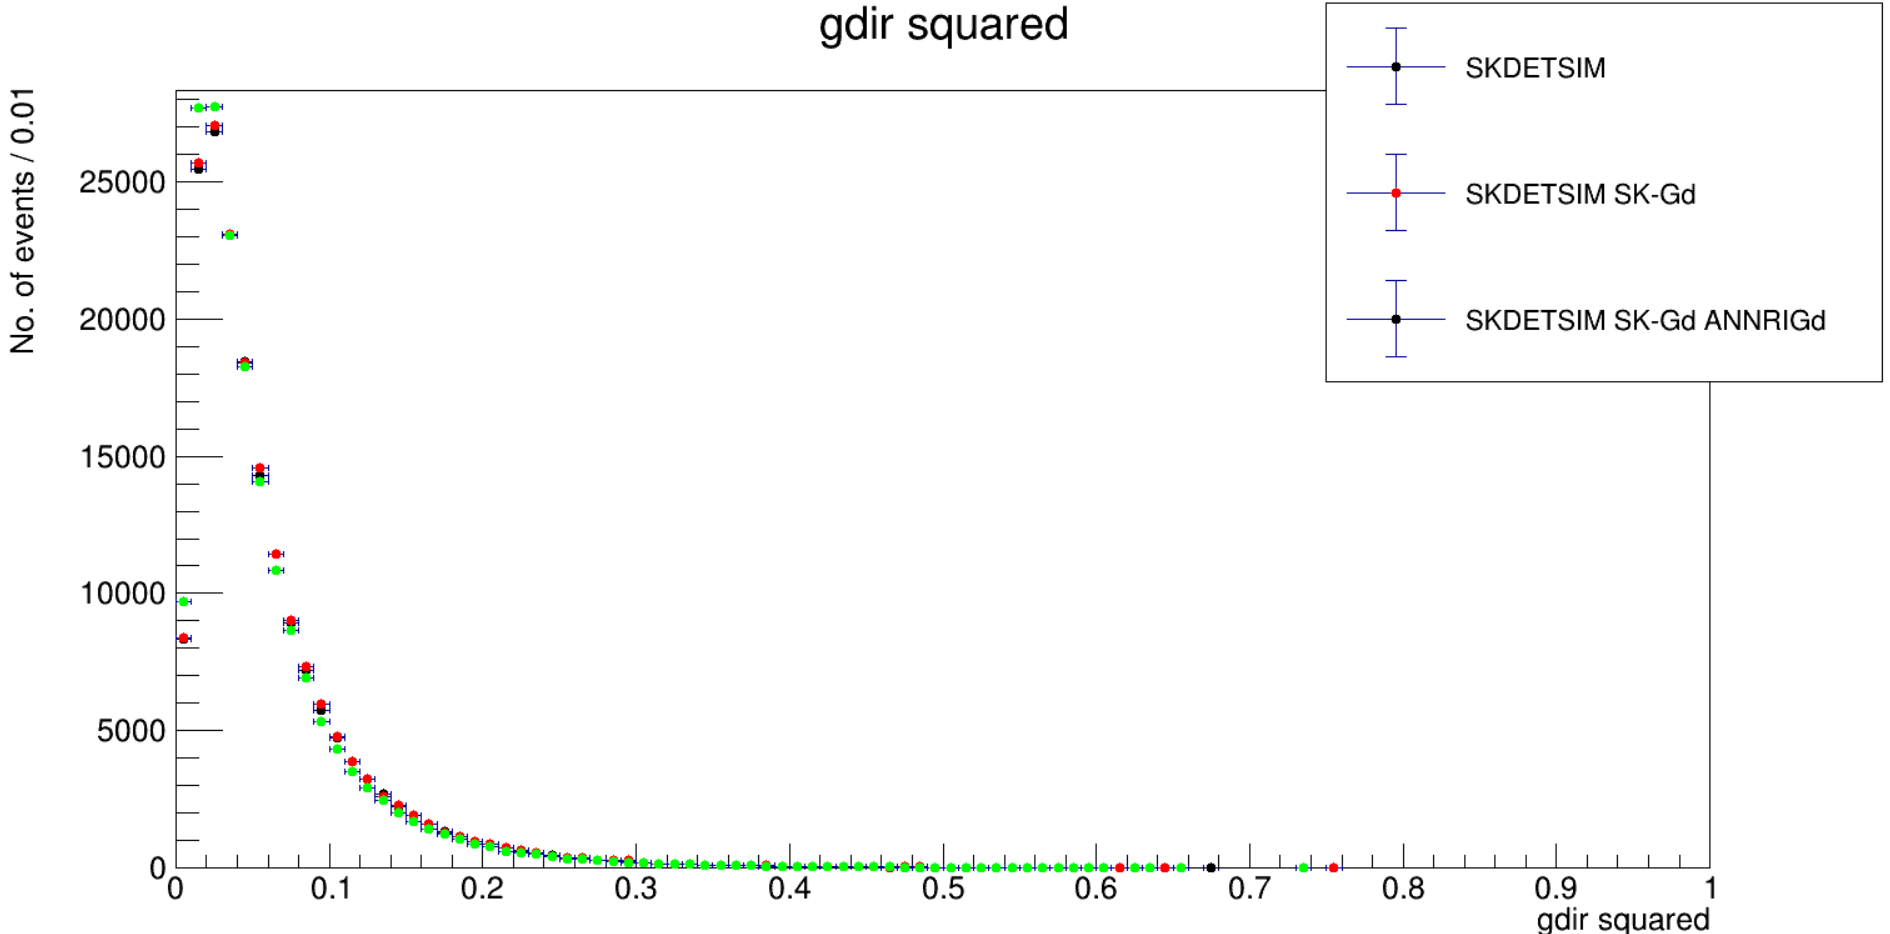
\includegraphics[width=0.49\textwidth]{Figures/gdir_squared.JPEG}} \label{fig:gdir_squared} \par
    
        
\end{figure}

The vertex goodness (gvtx) and directional goodness (gdir) squared comparisons are shown in Figures \ref{fig:gvtx_squared} and \ref{fig:gdir_squared}. Figure \ref{fig:gvtx_squared} shows a slight discrepancy between the SKDETSIM versions, but not enough to warrant further investigation. In addition to checking the previous BONSAI reduction phase quantities, the distance between the true neutrino vertex from the simulation and the neutrino vertex from the BONSAI reconstruction was also checked for the different SKDETSIM versions, shown in Figure \ref{fig:vertex_resolution}. Table \ref{table:vertex_resolution} shows the value of this distribution which encompasses 1-sigma (68\%) of the number of events: this value was very similar for all SKDETSIM versions.
\begin{figure}

    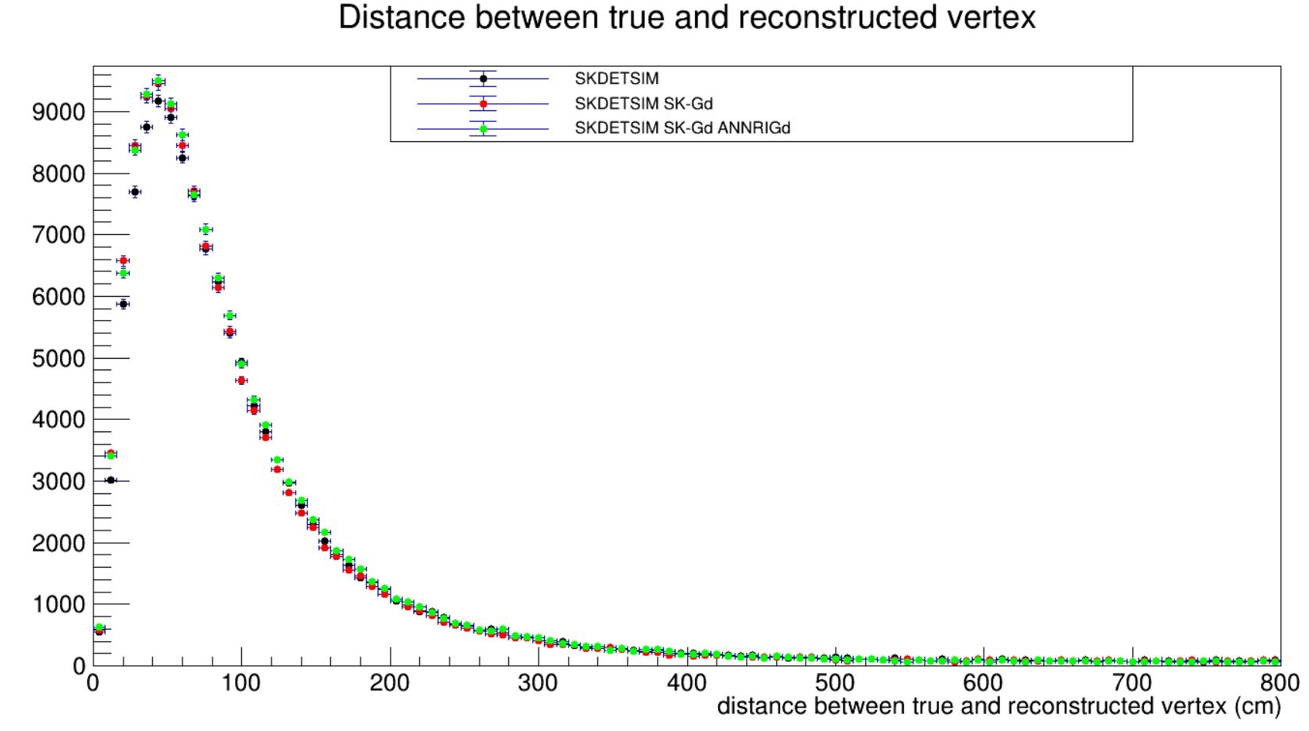
\includegraphics[width=\textwidth]{Figures/vertex_resolution.png}
    \caption{Distance between true and reconstructed neutrino vertex for different SKDETSIM versions}
    \label{fig:vertex_resolution}

\end{figure}

\begin{table}
    $$
    \begin{array}{rcc}
    \hline \text { SKDETSIM version } & \text{Value (cm)} \\
    \text{SKDETSIM-V} & 113.2\\
    \text{SKDETSIM-SKGd (Photon evaporation model)} & 109.4 \\
    \text{SKDETSIM-SKGd (ANNRI-Gd model)} & 111.9 \\
    \hline
    \end{array}
    $$
\caption{Value of the true neutrino vertex - reconstructed neutrino vertex distribution which encompasses 1-sigma (68\%) of the number of events.}
\label{table:vertex_resolution}
\end{table}

\subsubsection{Comparisons of event reconstruction output between NTag versions}
To ensure that the NCQE event selection and neutron tagging could be carried out using the new NTag code, comparisons of the output BONSAI reconstruction variables between the two versions were made to ensure the validity of the reconstruction output. Figures \ref{fig:energy_recon_compare}, \ref{fig:dwall_recon_compare}, \ref{fig:effwall_recon_compare}, \ref{fig:angle_recon_compare}, \ref{fig:ovaq_recon_compare} show the reconstructed energy, dwall, effwall, Cherenkov angle and ovaQ parameters respectively, with the legacy NTag output in black and the new NTag output in red. 

\begin{figure}[t!] % "[t!]" placement specifier just for this example
    \begin{subfigure}{0.48\textwidth}
    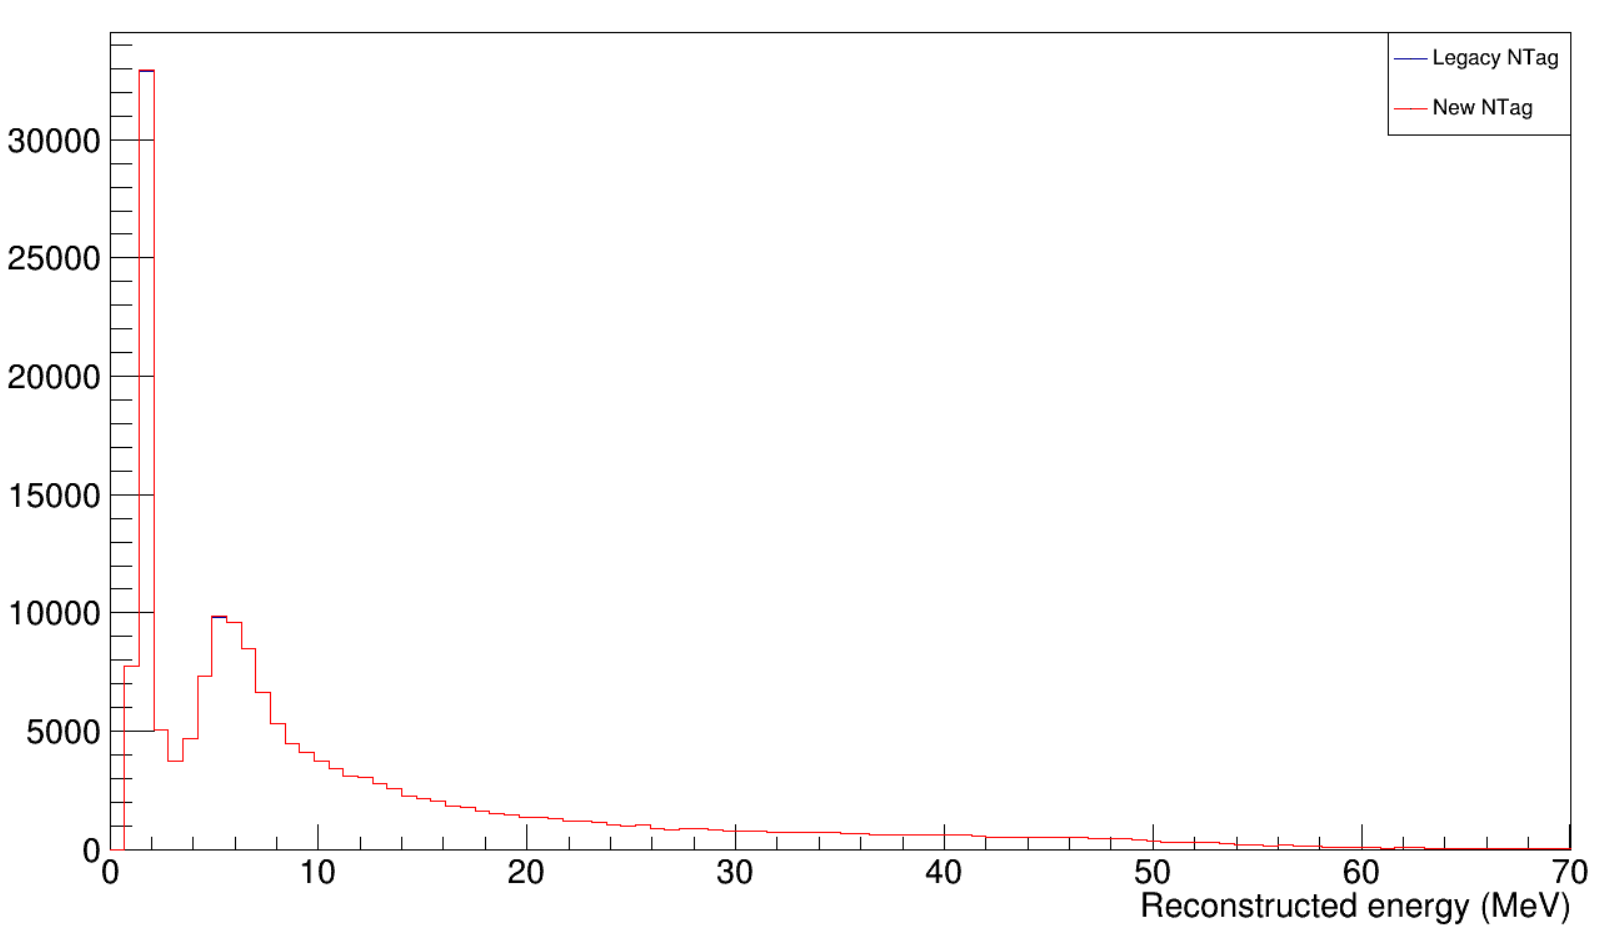
\includegraphics[width=\linewidth]{Figures/energy_recon_compare.PNG}
    \caption{Reconstructed energy (MeV) comparison} \label{fig:energy_recon_compare}
    \end{subfigure}\hspace*{\fill}
    \begin{subfigure}{0.48\textwidth}
    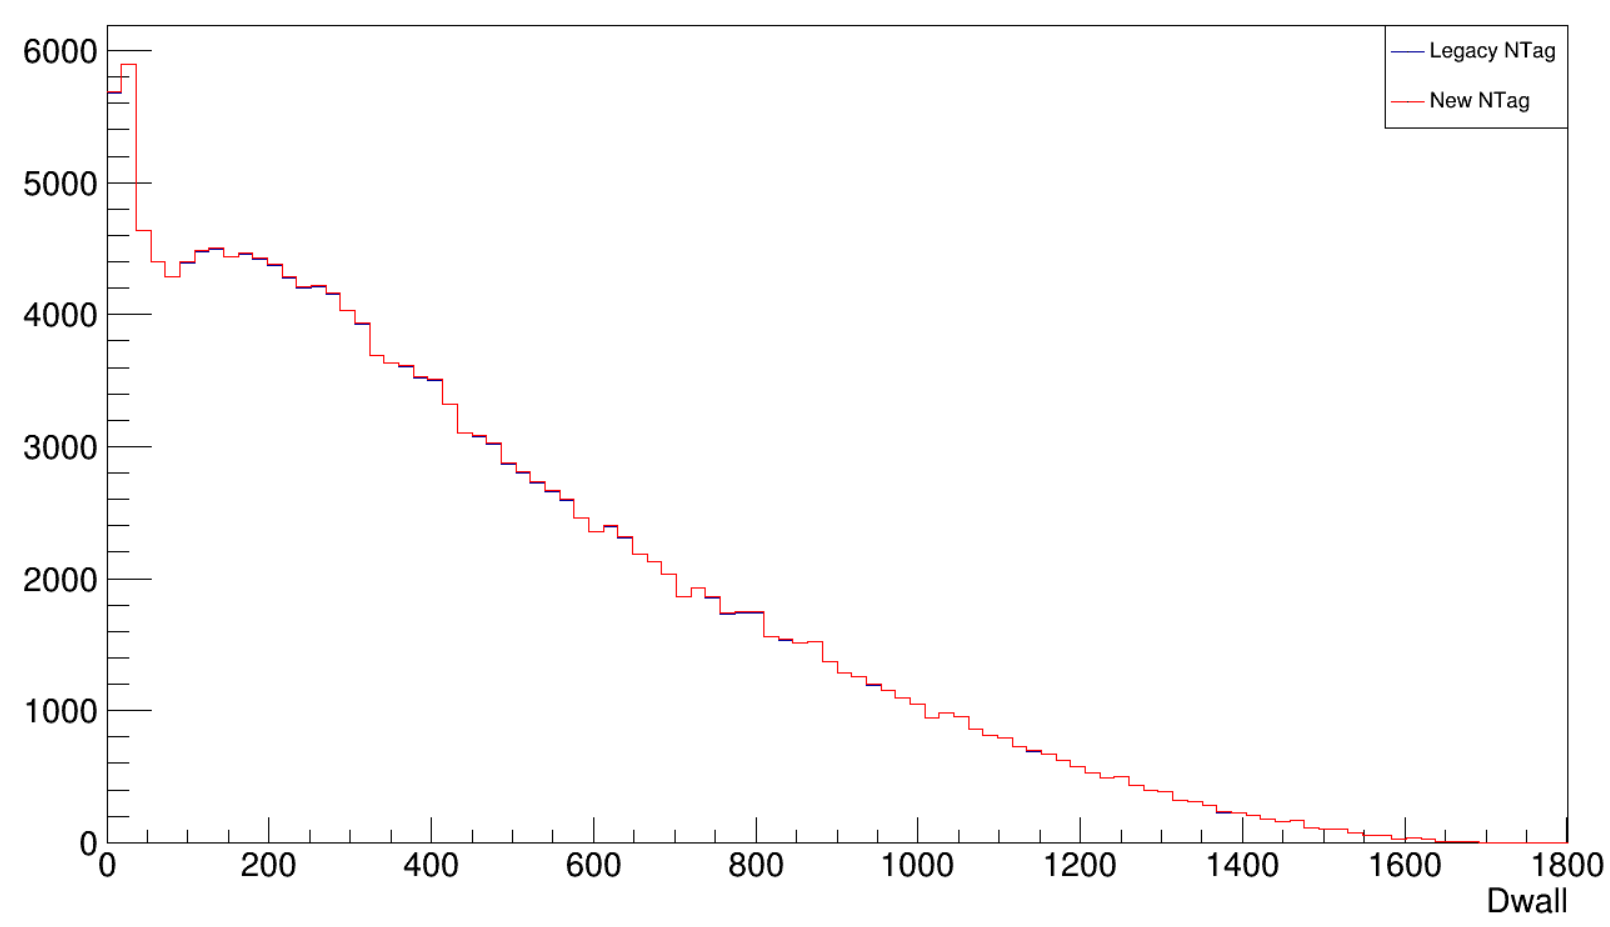
\includegraphics[width=\linewidth]{Figures/dwall_recon_compare.PNG}
    \caption{DWall (cm) comparison} \label{fig:dwall_recon_compare}
    \end{subfigure}
    
    \medskip
    \begin{subfigure}{0.48\textwidth}
    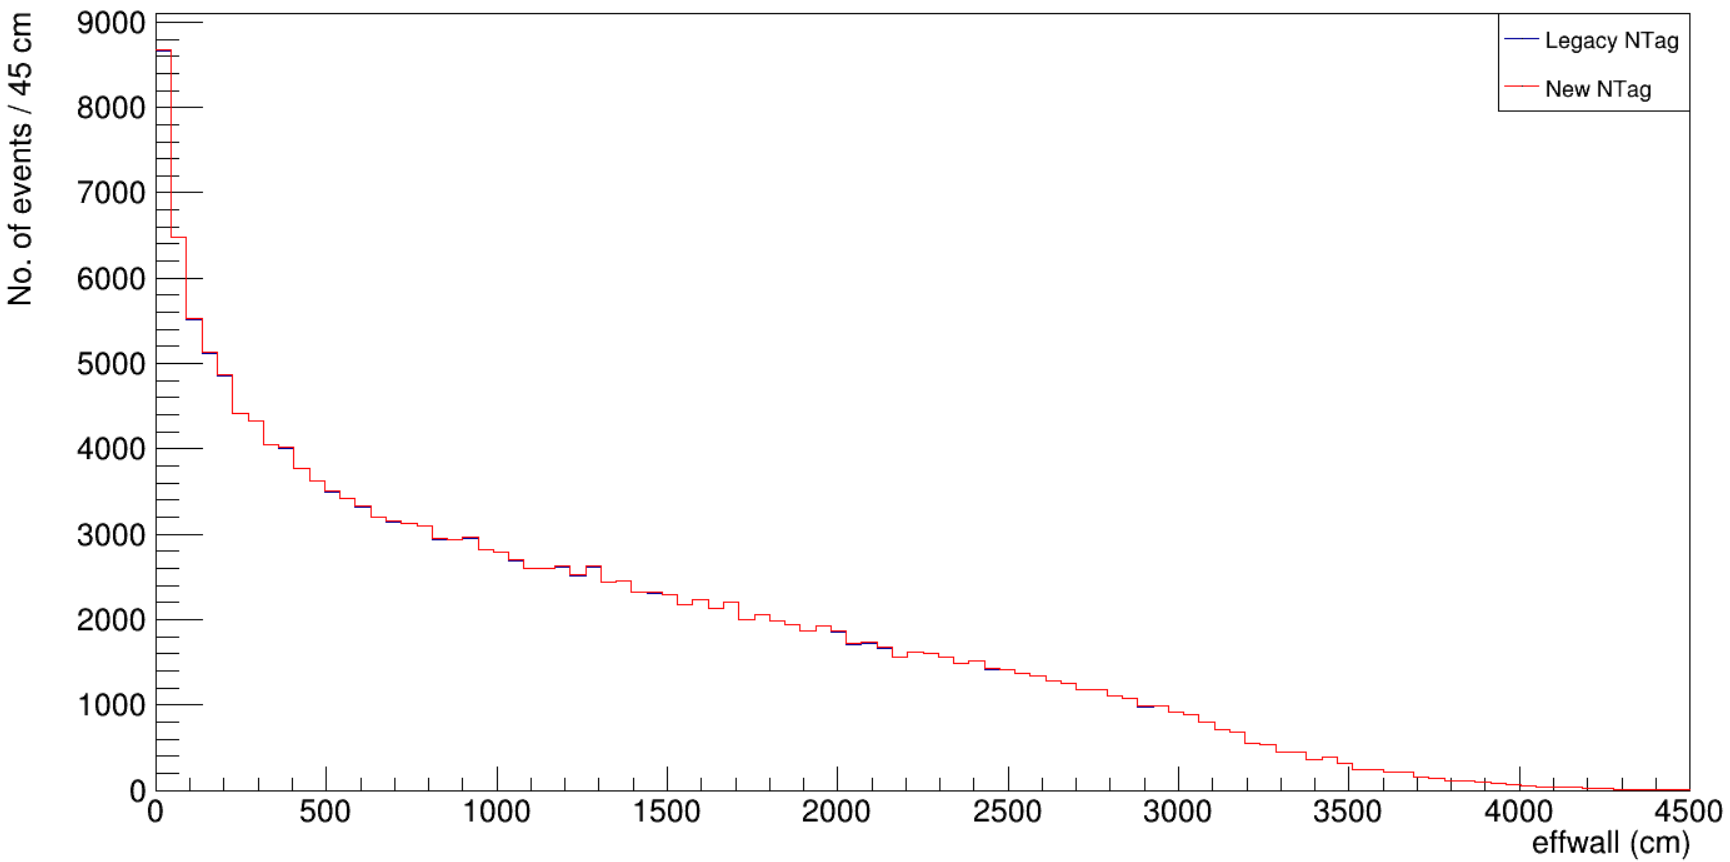
\includegraphics[width=\linewidth]{Figures/effwall_recon_compare.PNG}
    \caption{Effwall (cm) comparison} \label{fig:effwall_recon_compare}
    \end{subfigure}\hspace*{\fill}
    \begin{subfigure}{0.48\textwidth}
    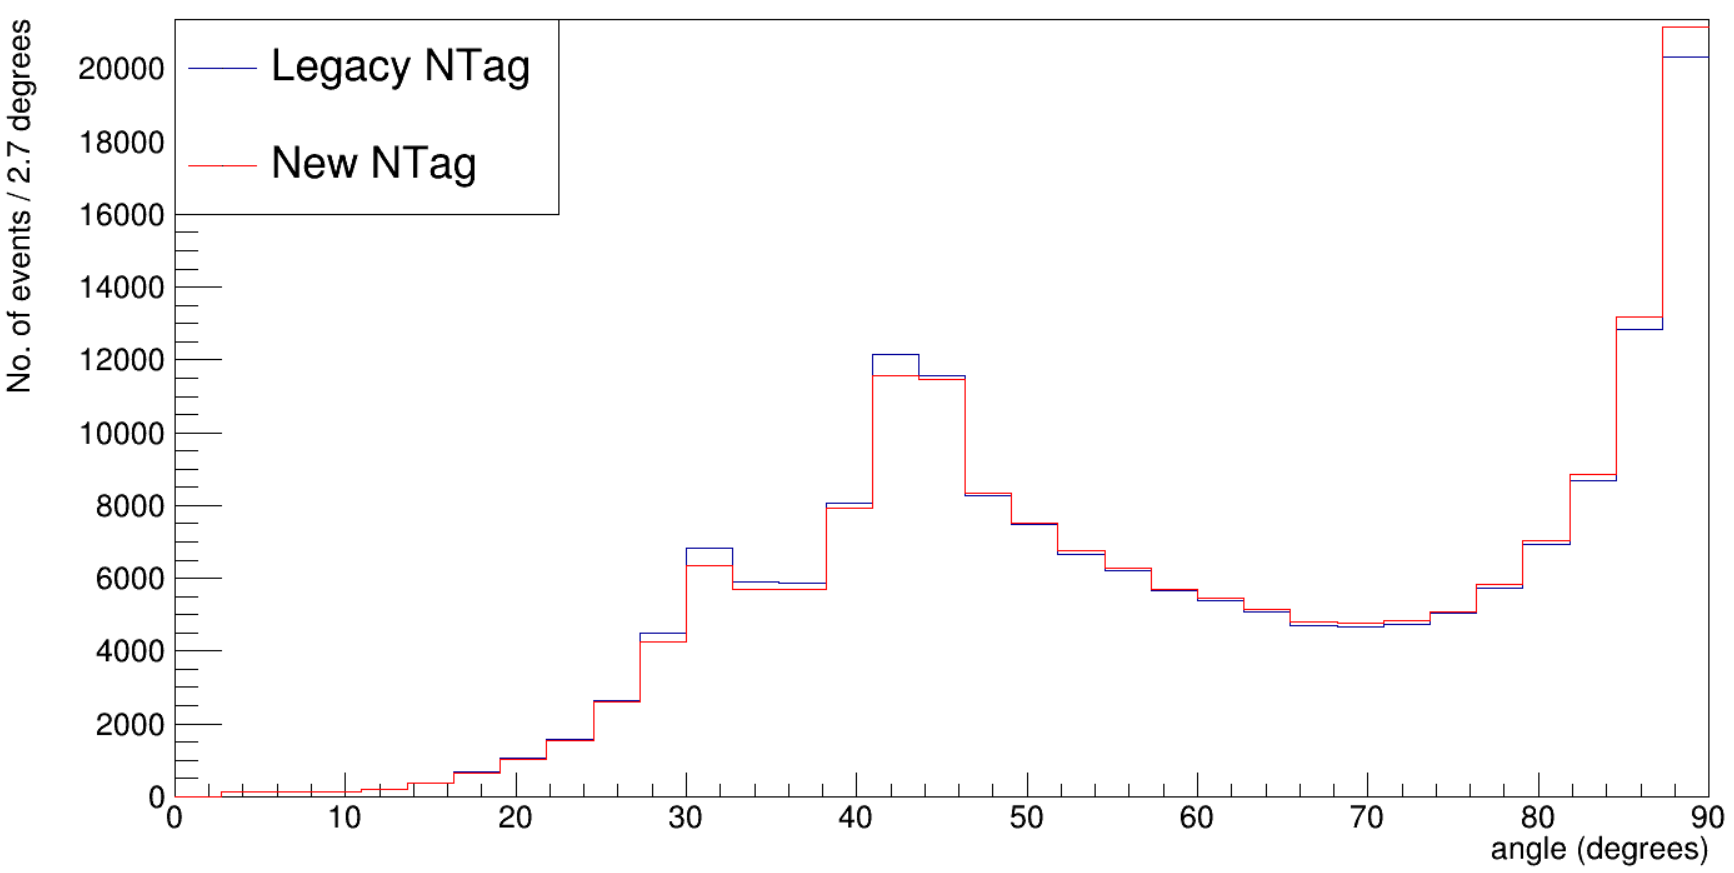
\includegraphics[width=\linewidth]{Figures/angle_recon_compare.PNG}
    \caption{Reconstructed Cherenkov angle (degrees) comparison} \label{fig:angle_recon_compare}
    \end{subfigure}
    
    \medskip
    \begin{subfigure}{0.48\textwidth}
    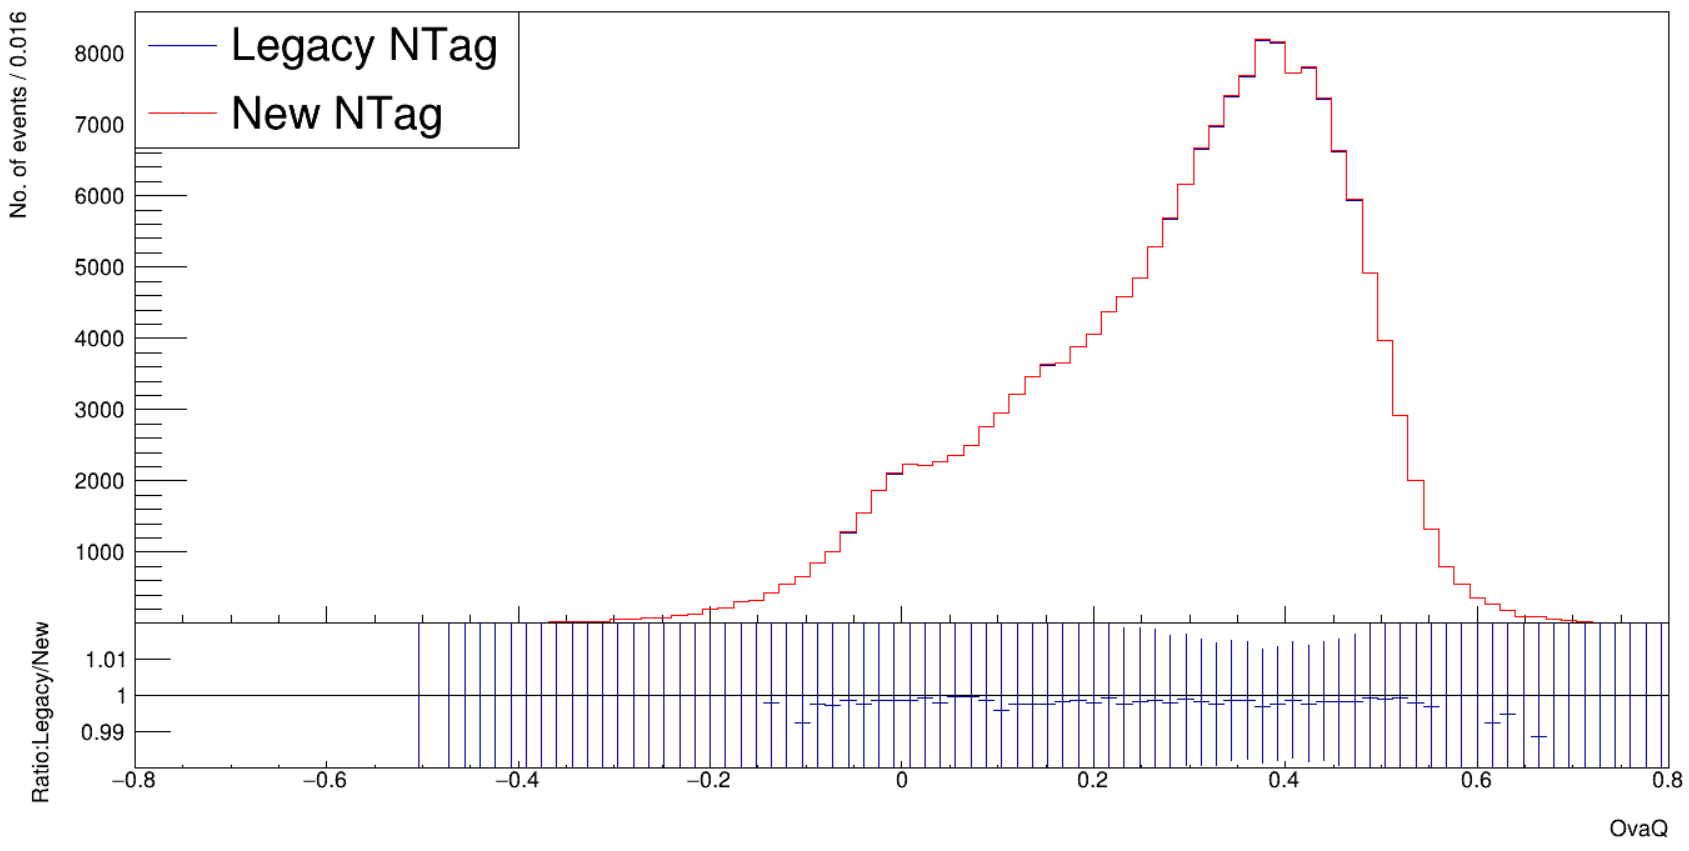
\includegraphics[width=\linewidth]{Figures/ovaq_recon_compare.PNG}
    \caption{OvaQ comparison} \label{fig:ovaq_recon_compare}
    \end{subfigure}\hspace*{\fill}
    
 
    \caption{Comparison of the output between the two NTag codes showing legacy (black) and new (red) NTag outputs}
    
    \end{figure}




\subsection{NCQE event selection}

Prior to applying the neutron tagging algorithm which searches for neutron candidates, events which satisfy the neutral current quasi-elastic criteria need to be selected. This selection only involves the neutrino vertex information, no information about the neutron candidates is used in the NCQE selection process. 
\newline
The following cuts are applied to the Monte Carlo, in order to select the NCQE events. These include a visible energy cut, a fiducial volume cut, a low energy background cut, and a cut to exclude charged currrent interaction events (CCQE). 

\subsubsection{Visible energy cut}
The energy window for this analysis is set to the 3.49-29.49 MeV range, where the lower value of this range (3.49 MeV) is due to the detection threshold of Super-Kamiokande. In order to limit the background of the Michel electron from charged-current interactions involving muon neutrinos and muon anti-neutrinos, the upper energy window limit is set to 29.49 MeV - above this value the Michel electron background would increase, reducing the NCQE contribution. 

\subsubsection{Fiducial Volume (FV) cut}
Due to radioactive impurities inside the detector material, specifically the wall of the inner detector, there is a cut involving the distance from the detector wall to the prompt interaction vertex. Events where the distance between the prompt interaction vertex and the detector wall is less than 200 cm are removed. There is a similar cut also used where events where the distance between the prompt interaction vertex and the distance to the inner detector wall in the neutrino vertex vector direction is less than 200 cm is removed. This is a standard cut applied in all Super-Kamiokande analyses in order to avoid backgrounds, and when you have events where the energy region is below 6 MeV even more stringent cuts are required to further reduce background from the inner detector wall, described in the next Subsection. 

\subsubsection{Low energy background cut}

The variables dwall, effwall and ovaQ are used to tune cuts in the energy region below 6 MeV. There are five energy regions with a width of 0.5 MeV used between the lower end of the visible energy cut region (3.49 MeV) and 5.99 MeV where the cuts on the dwall, effwall and ovaQ variables are optimised. Cuts are applied on the dwall, effwall and ovaQ variables and an event is only accepted if the values of dwall, effwall and ovaQ are only accepted if their values are greater than the threshold cut values. In each 0.5 MeV energy interval, these threshold values are optimised based on the T2K run period due to the beam power and detector conditions being different from run to run, especially since the Gadolinium loading occured in the detector. Equation \ref{eq:FOM} shows how the figure-of-merit (FOM) value is to be maximised for the optimsation of each cut.

\begin{equation}
    \mathrm{FOM}=\frac{N_{\text {sig }}}{\sqrt{N_{\text {sig }}+N_{\text {bkg }}}} \quad\left(N_{\text {bkg }}=N_{\text {bkg }}^{\mathrm{MC}}+N_{\text {bkg }}^{\text {beam-unrelated }}\right)
\label{eq:FOM}
\end{equation}

Here $N_{sig}$ is the number of NCQE neutrino events in the FHC Monte Carlo sample and $N_{bkg}$ is the summation of the background events, and the FOM is calculated seperately in the five energy intervals, and the optimised cut value is taken as the one which maximises the FOM. Then the optimised cut values in each energy interval are fitted with a linear function dependent on the visible energy variables (Erec). Equation \ref{eq:FOM_linear} gives the relation of Erec to the optimised cut values for dwall, effwall and ovaQ.

\begin{align}
    \text { dwall }^{\text {CUT }} =p_{0}^{\text {dwall }}+p_{1}^{\text {dwall }} \times E_{\text {rec }} \\
    \text { effwall }^{\text {CUT }}=p_{0}^{\text {effall }}+p_{1}^{\text {effwall }} \times E_{\text {rec }} \\
    \text { ova } Q^{C U T}=p_{0}^{\text {ovaQ }}+p_{1}^{\text {ovaQ }} \times E_{\text {rec }}
\label{eq:FOM_linear}
\end{align}


The scan regions and intervals for the dwall, effwall and ovaQ parameters for Equation \ref{eq:FOM_linear} are given in \cite{Abe_2019}. 

\subsection{Charged current event (CC) interaction cut}

In order to reduce the number of charged-current events which may be mistakenly included in the NCQE selection, a cut regarding the reconstructed Cherenkov angle of the prompt event  is also utilised alongside the low energy background cut, where the accepted Cherenkov angle of a prompt event ($theta_{C}$) should be greater than the threshold cut value $\theta_{C}^{CUT}$ where the cut value is determined by the linear equation dependent on Erec as shown in Equation \ref{eq:thetaC_FOM}.

\begin{equation}
    \theta_{C}^{C U T}=p_{0}^{\theta_{C}}+p_{1}^{\theta_{C}} \times E_{\text {rec }}
    \label{eq:thetaC_FOM} 
\end{equation}

Just like for the low energy background cut values, the values of the optimised parameters in Equation \ref{eq:thetaC_FOM} are given in \cite{Abe_2019}.


\subsection{Prompt event NCQE reduction cut plots}

Before applying the NTag algorithm, either legacy or new, plots were produced of the number of neutrino events and their dependence the reduction cut variables mentioned previously. These are shown in Figures \ref{fig:erec_reduction}, \ref{fig:dwall_reduction}, \ref{fig:effwall_reduction}, \ref{fig:angle_reduction}, \ref{fig:ovaq_reduction}. Each figure shows the corresponding plot for the previous NCQE analysis carried out with neutron tagging on Hydrogen on the left, with the plot from this analysis on the right. 


\begin{figure}[!htbp]
    \centering
    
    \caption{Comparisons of stacked histrograms for the Erec variable between NCQE neutron tag on H analysis (left) and this analysis (right)} \label{fig:erec_reduction} 
    
    \subfloat[]{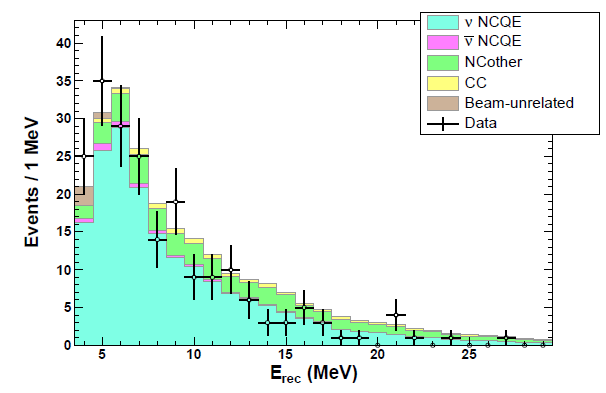
\includegraphics[width=0.49\textwidth]{Figures/fabio_erec.PNG}}  \hfill 
    \subfloat[]{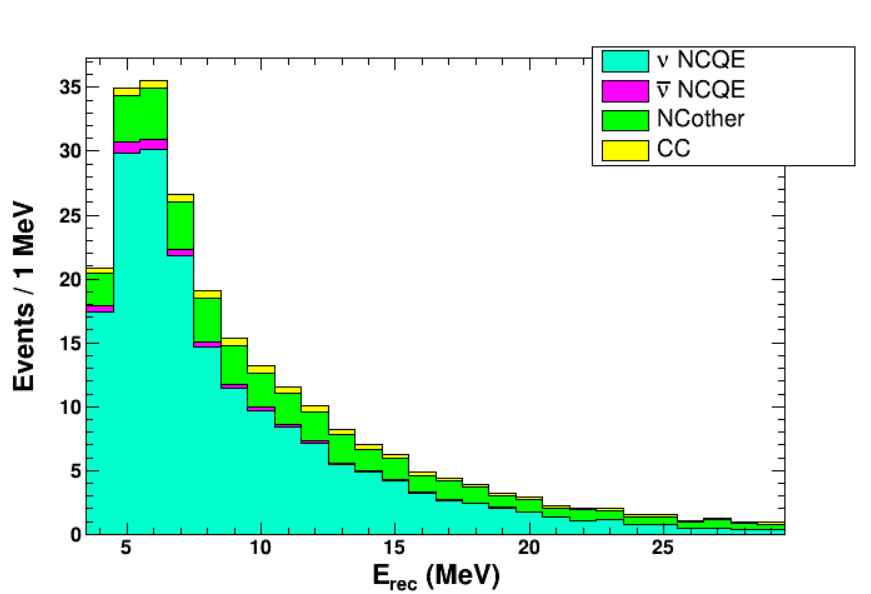
\includegraphics[width=0.49\textwidth]{Figures/erec_reduction.PNG}} \par
    
        
\end{figure}

\begin{figure}[!htbp]
    \centering
    
    \caption{Comparisons of stacked histrograms for the Dwall variable between NCQE neutron tag on H analysis (left) and this analysis (right)} \label{fig:dwall_reduction} 
    
    \subfloat[]{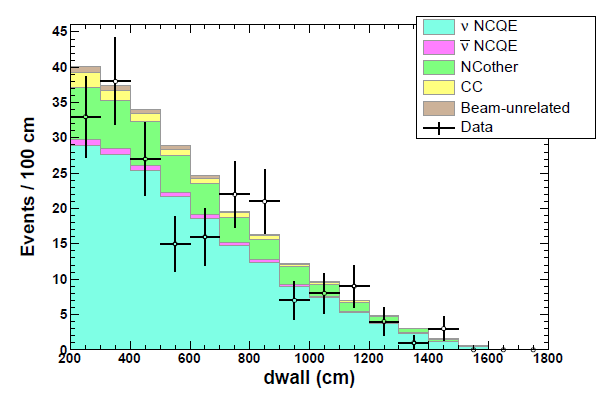
\includegraphics[width=0.49\textwidth]{Figures/fabio_dwall.PNG}}  \hfill 
    \subfloat[]{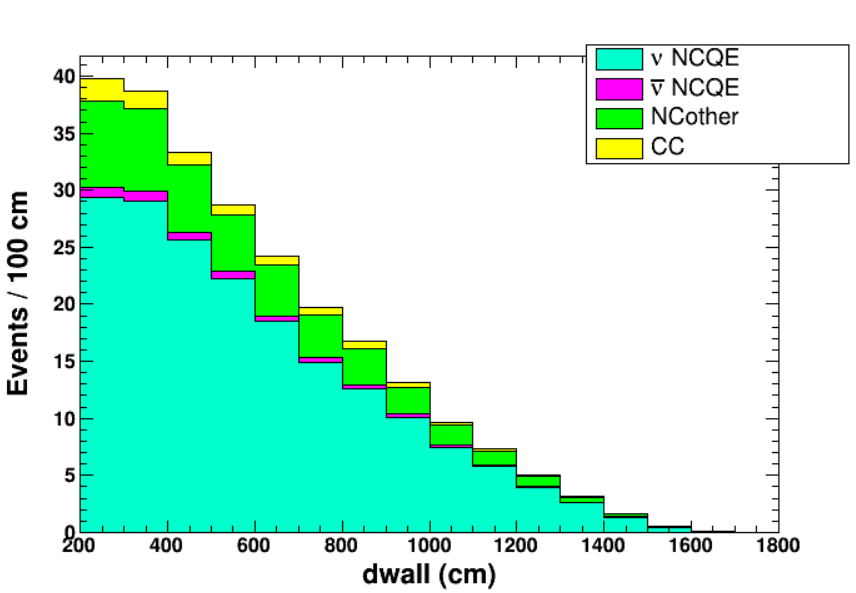
\includegraphics[width=0.49\textwidth, height=4.2cm]{Figures/dwall_reduction.PNG}}  \par
    
        
\end{figure}

\begin{figure}[!htbp]
    \centering
    
    \caption{Comparisons of stacked histrograms for the Effwall variable between NCQE neutron tag on H analysis (left) and this analysis (right)} \label{fig:effwall_reduction} 
    
    \subfloat[]{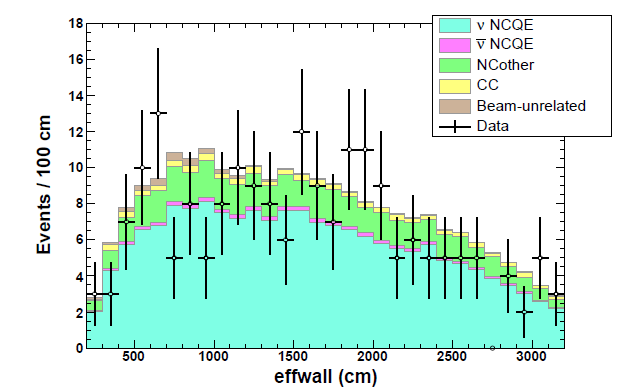
\includegraphics[width=0.49\textwidth]{Figures/fabio_effwall.PNG}}  \hfill 
    \subfloat[]{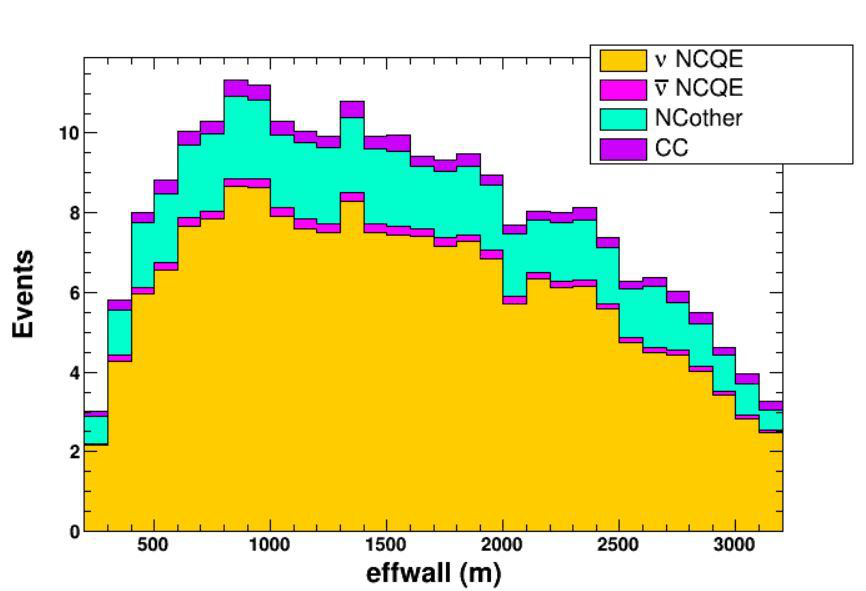
\includegraphics[width=0.49\textwidth]{Figures/effwall_reduction.PNG}} \par
    
        
\end{figure}

\begin{figure}[!htbp]
    \centering
    
    \caption{Comparisons of stacked histrograms for the ovaQ variable between NCQE neutron tag on H analysis (left) and this analysis (right)} \label{fig:ovaq_reduction} 
    
    \subfloat[]{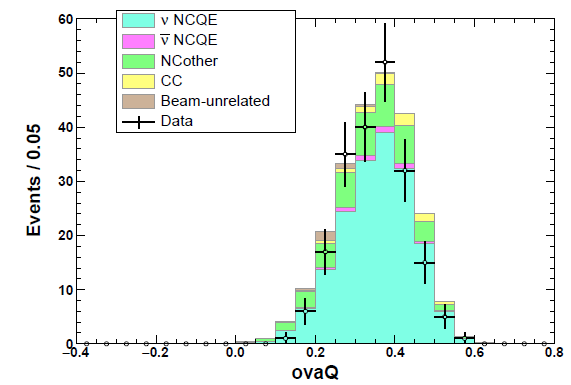
\includegraphics[width=0.49\textwidth]{Figures/fabio_ovaq.PNG}} \hfill 
    \subfloat[]{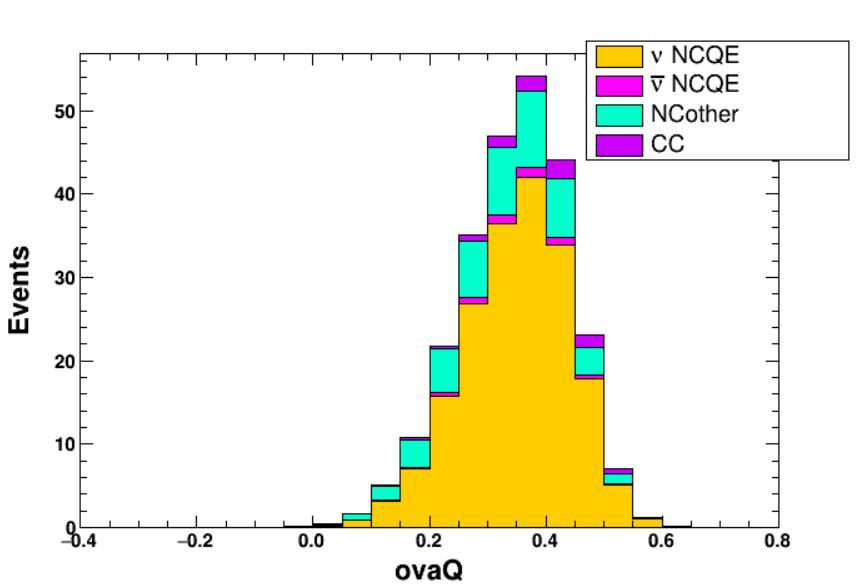
\includegraphics[width=0.49\textwidth]{Figures/ovaq_reduction.PNG}} \par
    
        
\end{figure}

\begin{figure}[!htbp]
    \centering
    
    \caption{Comparisons of stacked histrograms for the $\theta_C$ variable between NCQE neutron tag on H analysis (left) and this analysis (right)} \label{fig:angle_reduction} 
    
    \subfloat[]{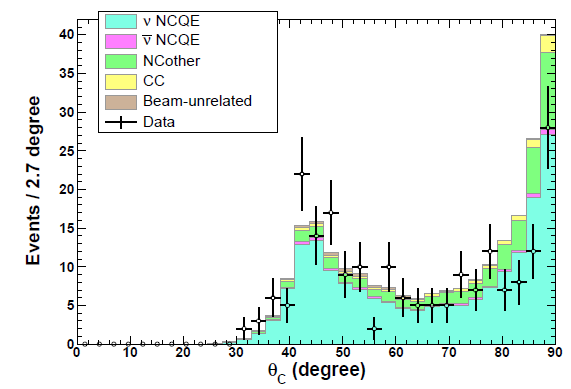
\includegraphics[width=0.49\textwidth]{Figures/fabio_angle.PNG}} \hfill 
    \subfloat[]{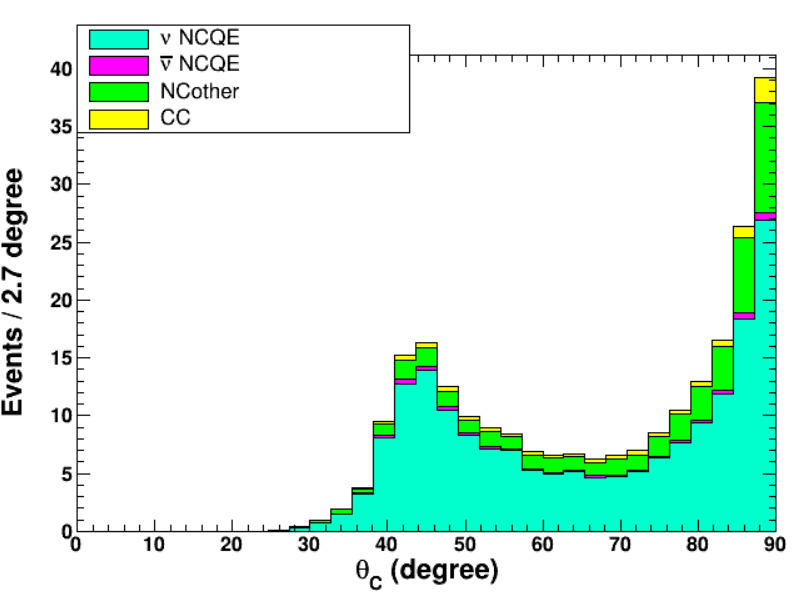
\includegraphics[width=0.49\textwidth, height=4.2cm ]{Figures/angle_reduction.PNG}} \par
    
        
\end{figure}






\subsection{True neutron tagging information}
\subsection{Primary selection criteria}
\subsection{Secondary selection criteria}
When the neutron vertex is found by this method, 14 variables which describe different aspects of the neutron candidate are calculated. For each of the neutron candidates the vector of these variables are computed and fed into the neural network and this produces an output value which is between 0 and 1. These variables relate to different features regarding categorising hits from neutron capture on Gd or H, including the number of the hits from neutron capture, the isotropy of these hits, the Cherenkov angles of these hits and the position of the neutron vertex in the detector when capture occurs. A description of these variables are given as follows:


\underline{N10nvx}
\newline
This is the number of hits in the 10ns sliding window of the neutron candidate
\newline


\underline{N300S}
\newline
Excluding the number of hits in the 10ns sliding window (N10nvx), this is the number of hits in the extended window of 300ns.
\newline


\underline{NcS}
\newline
This variable is defined as:
\begin{equation}
\label{ncs}
    NcS = N10nvx - Nclushit
\end{equation}

    Where $Nclushit$ is the number of clusterised hits: if hit \textit{i} and \textit{j} are hits on PMTs, then for hit \textit{i} and hit \textit{j} the hit vector $\hat{r}_i$ can be written as:

\begin{equation}
\label{hit}
    \hat{r}_{i}=\frac{\overrightarrow{P M T_{i}}-\overrightarrow{V T X_{n}}}{\left\|\overrightarrow{P M T_{i}}-\overrightarrow{V T X_{n}}\right\|}
\end{equation}

where the angle at the point of the neutron capture vertex between $\hat{r}_{i}$ and $\hat{r}_{j}$ of the PMT hits is defined as:

\begin{equation}
\theta_{i j}=\arccos \left(\hat{p}_{i} \cdot \hat{p}_{j}\right)
\end{equation}

where the hits are defined as clustered if $\theta_{ij}$ is less than 14


\underline{llrca}
\newline
This variable is the log likelihood ratio calculated using triplets of hits from N10nvx that make up a rudimentary Cherenkov cone, from which the opening angle $\theta$ is calculated. Two PDFs ($\theta_{Ci}$) and ($\theta_{Ci}$) are calculated from each $\theta_{Ci}$ where p\_s and p\_b are the probability density functions of $\theta_{C}$ depending on whether the hits come from a true neutron capture on Gd or H or a false neutron capture which makes up the background. The log likelihood ratio variable is computed using Equation {\ref{llrca}}.

\begin{equation}
\label{llrca}
\newline
  llrca =\sum_{i \in\{ { triplets }\}} \log \left(\frac{f_{B}\left(\theta_{C i}\right)}{f_{S}\left(\theta_{C i}\right)}\right)
\end{equation}


\underline{beta-n}
\newline
These variables (where n = 1,2,3,4,5) are defined using Legendre polynomials, shown in Equation \ref{beta}, which gives the isotropy of the Cherenkov hits.

\begin{equation}
\label{beta}
 beta- n=\frac{2}{N 10 {nvx}(N 10 {nvx}-1)} \sum_{i \neq j}  { Legendre }_{n}\left(\cos \theta_{i j}\right)
\end{equation}

where $Legendre_n$ gives the Legendre polynomial of order $n$ and $theta_{ij}$ is the angle between hit PMTs relative to the neutron capture vertex.



\underline{ndwall}
\newline
This parameter, similar to dwall, gives the shortest distance of the neutron capture vertex from the wall of the Super-Kamiokande tank.
\newline



\underline{ntowall}
\newline
This variable (similar to effwall), gives the distance of the neutron capture vertex from the wall, however, unlike ndwall it gives the direction of the neutron capture specifically along the direction of the centre of the hits. The direction ($\overrightarrow{R}$) is given by:

\begin{equation}
\overrightarrow{\operatorname{dir}}=\sum_{i=1}^{N 10 n v x} \hat{p}_{i}
\end{equation}





